% \documentclass[]{article}
\documentclass[13.5pt]{extarticle} 
\usepackage{hyperref} % 通常放在最后（少数宏包需在其后，如 cleveref）
\hypersetup{
    colorlinks=true,
    linkcolor=black,        % 默认链接颜色（包括目录）
    citecolor=blue,
    % urlcolor=red
}

% 或者更精细的控制（需要额外包）
\usepackage{xcolor}
\usepackage{hyperref}

% 定义不同颜色
\newcommand{\figref}[1]{\hypersetup{linkcolor=red}\ref{#1}}

\usepackage{booktabs}
\usepackage{tabularx}
\usepackage{makecell}
\usepackage{graphicx} % Required for inserting images
\usepackage{setspace}
% 引入中文支持包 (建议使用 XeLaTeX 编译)
\usepackage[UTF8]{ctex}
\usepackage{caption}

% 全局设置 caption 样式
\captionsetup{font=scriptsize}
\captionsetup{
    % font={small},            % 整体字体大小：small (小号), footnotesize (注脚大小)
    labelfont={bf},          % 标签字体（如"图1"）：bf (加粗), it (斜体)
    textfont={rm},           % 文本字体（如描述）：it (斜体), rm (罗马), sf (无衬线)
    labelsep=quad            % 标签与文本之间的分隔符：quad (空格), colon (冒号), period (句号)
}
\captionsetup{font={stretch=1.5}}
% 引入数学公式和符号包
\usepackage{amsmath}
\usepackage{amssymb}
\usepackage{amsfonts}
\usepackage{bm} % 用于加粗希腊字母等

% 页面边距设置
\usepackage{geometry}
% \geometry{left=2.5cm, right=2.5cm, top=2.5cm, bottom=2.5cm}
\usepackage{titlesec}

\renewcommand{\abstractname}{%
    \fontsize{16}{0}\selectfont  % 36pt字体，40pt行距
    摘\nolinebreak\hspace{\ccwd}要  % 防止换行
    \vspace{0.5cm}
}

    
% 列表环境设置
\usepackage{enumitem}
\begin{document}

\begin{titlepage}
    \centering
    \vspace*{-2.5cm} 
    % ========== Logo 行 ==========
    \begin{minipage}{0.5\textwidth}
        \raggedright
        % \centering
        
\includegraphics[width=0.8\linewidth]{figures/company_logo.png} \\
        % {\large \textbf{ABC科技有限公司}}
    \end{minipage}
    \hfill
    \begin{minipage}{0.35\textwidth}
        % \centering
        \raggedleft
        
\includegraphics[width=0.8\linewidth]{figures/university_logo.png} \\
        % {\large \textbf{XX大学实验室}}
    \end{minipage}
    
    \vspace{5cm}
    
    % ========== 报告标题 ==========
    {\Huge \textbf{基于强化学习的多智能体协同路径规划：算法研究与应用综述}} \\[1cm]
    
    % \rule{\textwidth}{2pt} \\[0.4cm]
    % {\Huge \textbf{项目名称或报告标题}} \\[0.4cm]
    % \rule{\textwidth}{2pt} \\[1cm]
    
    % {\Large 关于XXX技术的研发与应用} \\[2cm]
    
    \vspace{3cm}

    
    \begin{center}
        {\fontsize{12}{0} \textbf{香港理工大学}} \\[0.3cm]
        {\fontsize{12}{0} \textbf{互联网与移动计算实验室}} \\[0.3cm]
        {\fontsize{12}{0} \textbf{(Internet and Mobile Computing Laboratory, IMCL)}}
    \end{center}
    
    \vspace{4cm}
    
    % ========== 版本信息 ==========
    \begin{center}
         \begin{tabular}{ll}
            \textbf{版本：} & \textbf{v1.0} \\
            \textbf{日期：} & \textbf{2026年1月} \\
            % \textbf{文档编号：} & \textbf{IMCL-TR-2026-001} \\
        \end{tabular}
    \end{center}
    \vspace{2cm}

    
    \vfill
    
    % ========== 底部 ==========
    % {\small 
    %     本报告由ABC科技有限公司与XX大学联合发布 \\
    %     联系方式：contact@abctech.com | lab@university.edu
    % }

\end{titlepage}

\clearpage
\setstretch{1.75}

\begin{abstract}
随着工业 4.0 与智慧物流的快速发展，大规模多智能体系统（MAS）的协同作业已成为提升生产效率的关键。多智能体路径规划（MAPF）作为 MAS 的核心决策模块，面临着从静态封闭环境向动态开放环境迁移的巨大挑战。传统基于搜索与规则的算法在处理高维状态空间、复杂动态交互及非确定性干扰时，往往遭遇维数灾难与实时性瓶颈。深度强化学习（DRL）凭借其强大的端到端感知与自适应决策能力，为解决大规模协同规划难题提供了全新的范式。

本报告系统综述了基于强化学习的多智能体协同路径规划算法及其应用研究。首先，报告回顾了传统 MAPF 方法并指出了其在可扩展性与鲁棒性上的局限，进而建立了基于 Dec-POMDP 的多智能体决策数学模型。其次，深入剖析了“集中训练-分散执行”（CTDE）架构下的主流算法范式：重点阐述了以 VDN、QMIX 为代表的值分解方法在解决离散空间信贷分配与死锁问题上的机制，以及以 MADDPG、MAPPO 为代表的策略梯度方法在连续空间动力学控制中的演进。此外，报告探讨了融合传统规划先验知识与强化学习探索能力的混合式架构（Hybrid Planning-Learning），以及基于图神经网络（GNN）的时空交互拓扑建模技术。最后，报告总结了当前算法在从仿真迁移至真实物理环境、安全性保障及大规模异构集群调度方面面临的挑战，并展望了其在无人驾驶商用车队及智能仓储系统中的应用前景。
\end{abstract}
\clearpage


\tableofcontents

\clearpage
\section{引言}

\subsection{研究背景与应用动机}

随着人工智能与自动化技术的飞速发展，多智能体系统（Multi-Agent Systems, MAS）已逐渐从理论研究走向大规模工业应用，其中多智能体路径规划（Multi-Agent Path Finding, MAPF）作为该系统的核心决策模块，其重要性日益凸显。MAPF问题的基本定义是在给定的环境中，为一组智能体分别规划出从各自起点到终点的最优路径，同时确保智能体之间以及智能体与静态障碍物之间不发生碰撞，并尽可能优化全局的运行时间或总移动成本。这一问题不仅是计算机科学与运筹学领域的经典难题，更是实现群体智能落地的关键技术支撑。根据最新的综述研究指出~\cite{alkazzi2024comprehensive}，尽管MAPF问题在图上的最优求解已被证明是NP-Hard的，但现代研究正致力于分析其在更复杂约束下的计算复杂性，这意味着随着智能体数量的增加，求解空间的复杂度呈指数级爆炸。然而，现实应用场景却恰恰要求算法能够应对大规模、高动态的智能体群体，并满足实时、安全的在线决策需求。理论与现实需求之间的这一根本矛盾， 使得工业4.0的柔性产线调度与智慧城市的实时交通流管理等场景中的协同路径规划，成为一个兼具可扩展性、实时性与安全性的严峻工程挑战，这也是实现物理系统与数字决策深度融合必须攻克的关键难题。

MAPF技术的应用动机源于现代物流、智能交通及机器人集群领域的迫切需求，其中最具代表性的应用场景莫过于智能仓储系统。以Amazon Robotics和阿里云物流为代表的自动化仓储系统，部署了成百上千台自动导引车或自主移动机器人在密集货架间穿梭，传统的固定轨道或分区控制已无法满足海量订单带来的高并发吞吐需求，系统必须依赖高效的协同规划算法来防止死锁并最大化分拣效率~\cite{okumura2023lacam}。此外，在自动驾驶领域，随着车辆网联化技术的发展，传统的交通信号灯控制正逐步向基于协同规划的无信号灯路口通行演进，车辆需要在毫秒级的时间窗口内协商路权以实现无碰撞穿插。同样，在低空经济领域，无人机集群编队在执行协同巡检、安防监控或灯光秀表演时，面临着更为严苛的三维空间避障与编队保持要求。这些典型场景共同指向了一个核心诉求：算法不仅要解决可达性问题，更要解决复杂约束下的时空协同问题。

然而，尽管经典算法在静态环境下已取得显著成果，但现实物理世界的复杂性为协作路径规划带来了严峻的理论与工程挑战。首先是环境的动态性与非确定性。在真实场景中，智能体的动作执行往往存在误差，且环境中可能存在不可预测的动态障碍物，这导致基于完美模型假设的传统搜索算法（如 A* 或 CBS）生成的预计算路径极易失效，频繁的重规划会造成计算资源的剧烈消耗与系统卡顿。其次是部分可观测性的约束。受限于传感器视场角和通信带宽，单个智能体往往无法获取全局的精确状态信息，必须在信息缺失的情况下仅凭局部观测做出最优决策~\cite{rashid2018qmix}。这种去中心化的决策模式虽然降低了对中央服务器的依赖，但也极易导致局部最优解或群体的非理性行为，例如活锁或震荡。因此，如何在通信受限、感知存在噪声且环境高度动态的约束下，保证多智能体系统的鲁棒性与安全性，是当前学术界与工业界共同面临的难题。

回顾MAPF领域的发展历程，可以清晰地看到从集中式搜索向解耦与协同演进的脉络。早期的研究主要集中在基于搜索的完备性算法，如Silver提出的协作A*（Cooperative A*, CA*）以及后来的基于冲突搜索（Conflict-Based Search, CBS）~\cite{everett2018motion}。CBS算法通过将多智能体路径规划问题分解为受约束的单智能体路径规划问题，在求解最优解方面取得了里程碑式的突破，但在面对密集障碍物或大规模集群时，其底层的冲突树规模仍会迅速膨胀，最新研究也指出也指出了其在终身任务场景下的扩展性瓶颈~\cite{chan2024anytime}。为了提升实时性，基于优先级的解耦方法和基于速度障碍物的反应式方法（如 ORCA）应运而生，这类方法虽然牺牲了路径的最优性以换取计算效率，但在复杂死锁场景下缺乏协同脱困能力。近年来，随着应用场景对算法适应性和泛化能力要求的提高，单纯依赖几何规则或启发式搜索的传统范式逐渐显露出局限性，这也促使研究者将目光投向了具备自适应学习能力的强化学习领域（Reinforcement Learning, RL），试图通过数据驱动的方式通过试错来习得复杂的协同策略。
\subsection{RL在路径规划中的优势}

传统的路径规划算法虽然在静态与完全已知的环境中能够保证完备性，但在面对现代复杂系统的动态性与高维特征时，往往显得力不从心。强化学习（RL），特别是深度强化学习，通过将感知与决策深度融合，为解决上述难题提供了全新的范式。与依赖精确环境建模的传统规划不同，RL采用无模型的学习机制，允许智能体通过与环境的持续交互试错来直接优化策略函数。这种机制赋予了系统极强的泛化能力与鲁棒性，使得智能体能够从原始的高维传感器输入，例如激光雷达点云或相机图像中直接提取空间特征并输出控制指令，实现了从感知到动作的端到端映射。Mnih 等人~\cite{mnih2015human}的研究表明，深度神经网络强大的函数拟合能力能够有效克服状态空间的维数灾难，使得在传统方法中无法建模的复杂动态障碍物交互成为可解问题。这意味着，基于RL的规划器不再需要预先存储一张完美的全局地图，而是具备了在未知环境中实时应对突发扰动  的类人直觉反应能力。

随着研究重心从单体智能转向群体智能，多智能体强化学习（MARL）的兴起进一步解决了协同规划中的核心矛盾——环境非平稳性与通信瓶颈。在单智能体 RL中，其他智能体通常被视为环境背景的一部分，但在多智能体系统中，所有智能体同时更新策略会导致环境状态转移概率随时间剧烈波动，使得独立学习难以收敛。MARL引入了博弈论的视角，特别是集中训练分布式执行架构的提出，彻底改变了这一局面。Lowe等人提出的MADDPG算法~\cite{lowe2017multi}展示了如何利用全局信息在训练阶段稳定 Critic 网络，而在执行阶段仅依赖局部观测让Actor 网络做出决策。这种架构不仅保留了分布式系统的高扩展性与低通信延迟优势，还通过在训练中引入显式的信用分配机制，解决了基于规则的解耦方法中常见的懒惰智能体或死锁问题。Rashid等人~\cite{rashid2018qmix}的研究进一步证实，通过值分解技术，MARL 能够让智能体群组自发涌现出复杂的战术配合（如交替通行、编队保护），而无需人工编写繁琐的规则库。
此外，在计算效率与在线实时性方面，强化学习展现出了相对于传统搜索算法的压倒性优势。传统的耦合规划算法属于在线计算密集型，其计算时间随着智能体数量呈指数级增长，一旦环境发生微小变化触发重规划，系统往往会因为计算超时而卡顿。相反，强化学习属于离线训练密集型，其繁重的计算负载被前置到了离线训练阶段。一旦模型训练完毕，在线部署时的路径规划过程仅涉及神经网络的前向推理，其时间复杂度通常为常数级或与邻居数量呈线性关系。Everett等人~\cite{everett2018motion}在多机器人防撞任务中的实验表明，基于RL的算法能够在毫秒级的时间窗口内为数十个机器人生成无碰撞的速度矢量，这种极致的响应速度对于自动驾驶车队、无人机集群等对延迟敏感的高动态系统而言，是传统规划方法难以企及的。因此，RL不仅提升了规划的灵活性，更为大规模集群的实时全局调度提供了可行的技术路径。
\subsection{国内外研究现状简述与代表性工作}
在多智能体路径规划的传统研究领域，以南加州大学的Sven Koenig教授团队为代表的学术力量长期占据主导地位，确立了基于搜索的算法基准。该团队提出的基于冲突搜索（CBS）算法彻底改变了以往将 MAPF 视为最大流问题或多商品流问题的求解思路，通过双层搜索架构实现了最优解的高效计算。随后，为了应对大规模场景下的计算瓶颈，Koenig团队与其合作者进一步提出了ECBS（Bounded Sub-optimal CBS）、CBSH（CBS with Heuristics）等变体，试图在最优性与计算速度之间寻找平衡~\cite{sharon2015conflict}。这一阵营的研究侧重于算法的理论完备性分析与组合优化边界的探索，其成果广泛应用于静态环境下的仓储调度，但在处理非结构化动态环境及传感器噪声方面，传统搜索算法的鲁棒性始终是难以突破的短板，这为引入数据驱动的方法留下了巨大的创新空间。

随着深度学习浪潮的兴起，国际上以麻省理工学院、牛津大学和卡内基梅隆大学为首的研究机构开始引领基于强化学习的协同规划潮流。麻省理工学院的 Jonathan How教授团队最早将深度强化学习应用于机器人避障，提出了CADRL（Collision Avoidance with Deep RL）及其后续的 GA3C-CADRL 框架~\cite{chen2017socially}，证明了端到端的神经网络能够直接从雷达数据中学习到复杂的社会化避让行为，实现了完全去中心化的实时规划。与此同时，牛津大学的Shimon Whiteson团队深耕于多智能体强化学习的底层机制，其提出的QMIX算法通过单调性约束巧妙地解决了值函数分解难题，成为当前协作型多智能体任务（如星际争霸II微操）的事实标准~\cite{rashid2018qmix}。卡内基梅隆大学的Howie Choset团队则致力于连接这两个世界，他们提出的PRIMAL框架创新性地结合了模仿学习与强化学习，利用传统规划器的专家数据引导RL智能体收敛，成功解决了大规模同构集群的冷启动与稀疏奖励问题~\cite{sartoretti2019primal}。这些开创性工作标志着MAPF研究范式从基于规则的几何计算向基于数据的交互学习发生了根本性转移。

近年来，国内高校与科研机构在多智能体系统与无人集群领域的研究也呈现出井喷式发展态势，迅速缩小了与国际顶尖水平的差距。以清华大学、北京大学、中国科学院自动化研究所以及天津大学为代表的科研团队，不仅在MARL 的基础理论（如通信机制、探索策略）上取得了显著突破，更在应用层面展现出独特的优势。例如，清华大学团队在基于图神经网络（GNN）的协同规划方面进行了深入探索，利用图注意力机制解决变规模智能体群组的交互建模问题~\cite{wang2020learning, liu2020multi}；中科院自动化所则聚焦于复杂博弈环境下的策略演化与对抗学习，推动了无人机集群在动态对抗场景下的实战化应用~\cite{zhang2019hierarchical, hu2020voronoi}。此外，国内的大型科技公司，阿里、华为、京东等依托其庞大的物流仓储与自动驾驶业务场景，发布了一系列基于大规模真实数据的 MAPF 挑战赛与数据集，推动了产学研的深度融合~\cite{li2021lifelong, zhou2020smarts}，使得国内研究更侧重于解决高密度、高并发与强干扰环境下的工程落地难题。

总体而言，当前MAPF领域的研究呈现出传统规划与深度学习双轨并行、互补融合的格局。一方面，基于搜索的方法依然是静态环境下追求最优解的首选，并在理论分析上提供了坚实的基础；另一方面，基于强化学习的方法凭借其强大的泛化能力与在线推理速度，正在成为解决高动态、部分可观测及连续控制问题的核心手段。未来的研究趋势正逐渐从单一范式向混合范式演进，即利用学习算法来加速搜索过程，或利用规划算法来约束学习策略，旨在构建兼具完备性保证与实时自适应能力的下一代协同规划系统。

\subsection{本文研究范围、贡献与创新点}

本文的研究范围聚焦于多智能体协同路径规划这一核心问题，重点探讨在环境动态性、感知不确定性及通信受限等复杂现实约束下，基于强化学习及其变体，特别是多智能体强化学习的解决方案。研究内容涵盖了从离散网格环境下的仓储机器人调度到连续物理空间中的无人车队动力学控制，系统地梳理了从基于值函数的离散决策到基于策略梯度的连续控制，再到融合传统规划的混合式架构的完整技术路线。本文的主要学术贡献在于建立了一个多维度的算法分类与评估体系，不仅从算法原理上对比了集中训练-分散执行（CTDE）与传统解耦规划的优劣，还深入剖析了不同通信拓扑与奖励机制设计对群体协同行为涌现的内在影响，填补了现有综述在算法理论与工程落地之间缺乏深度关联分析的空白。

与既往综述仅仅关注算法性能指标不同，本文的独特创新点在于提出了面向无人驾驶商用车队及全局调度系统的应用级技术框架。针对港口集装箱运输、矿山自动驾驶运输等特定的商用车队场景，本文探讨了如何将MAPF算法从二维平面的避障扩展为包含时间窗约束、车辆动力学约束及社会化交通规则约束的高维时空规划问题。特别是针对全局调度系统，本文提出了一种分层递阶的协同范式，即在上层利用图神经网络进行宏观的交通流预测与任务分配，在下层利用强化学习处理微观的车辆交互与博弈。这种面向商用级大规模集群的视角，不仅解决了传统算法在异构车队混行时的适应性难题，更为解决开放场景下无人驾驶车队的效率-安全平衡问题提供了具有前瞻性的理论支撑与实施路径。

基于上述研究背景与目标，本文的后续章节安排如下：第二章首先回顾基于搜索与规则的传统MAPF方法，并系统分析其在可扩展性与在线实时性方面面临的固有局限，为引入学习型方法奠定逻辑基础。第三章对多智能体路径规划问题进行严格的数学建模，定义 Dec-POMDP 框架及关键约束，并给出本文的算法分类体系。第四章与第五章构成本文的核心算法部分，分别详细阐述基于值函数分解的方法在离散调度中的应用，以及基于策略梯度的方法在连续控制中的演进。第六章探讨融合传统规划与强化学习的混合式架构，分析模仿学习与安全盾机制如何解决冷启动与安全性难题。第七章建立统一的实验评估标准，对各类算法在典型场景下的性能进行横向对比分析。最后，第八章总结全文，剖析当前面临的Sim-to-Real迁移、通信瓶颈等开放性挑战，并展望工业应用前景与未来发展方向，如图\figref{fig:outline}。

\begin{figure}[htbp]
    \centering
    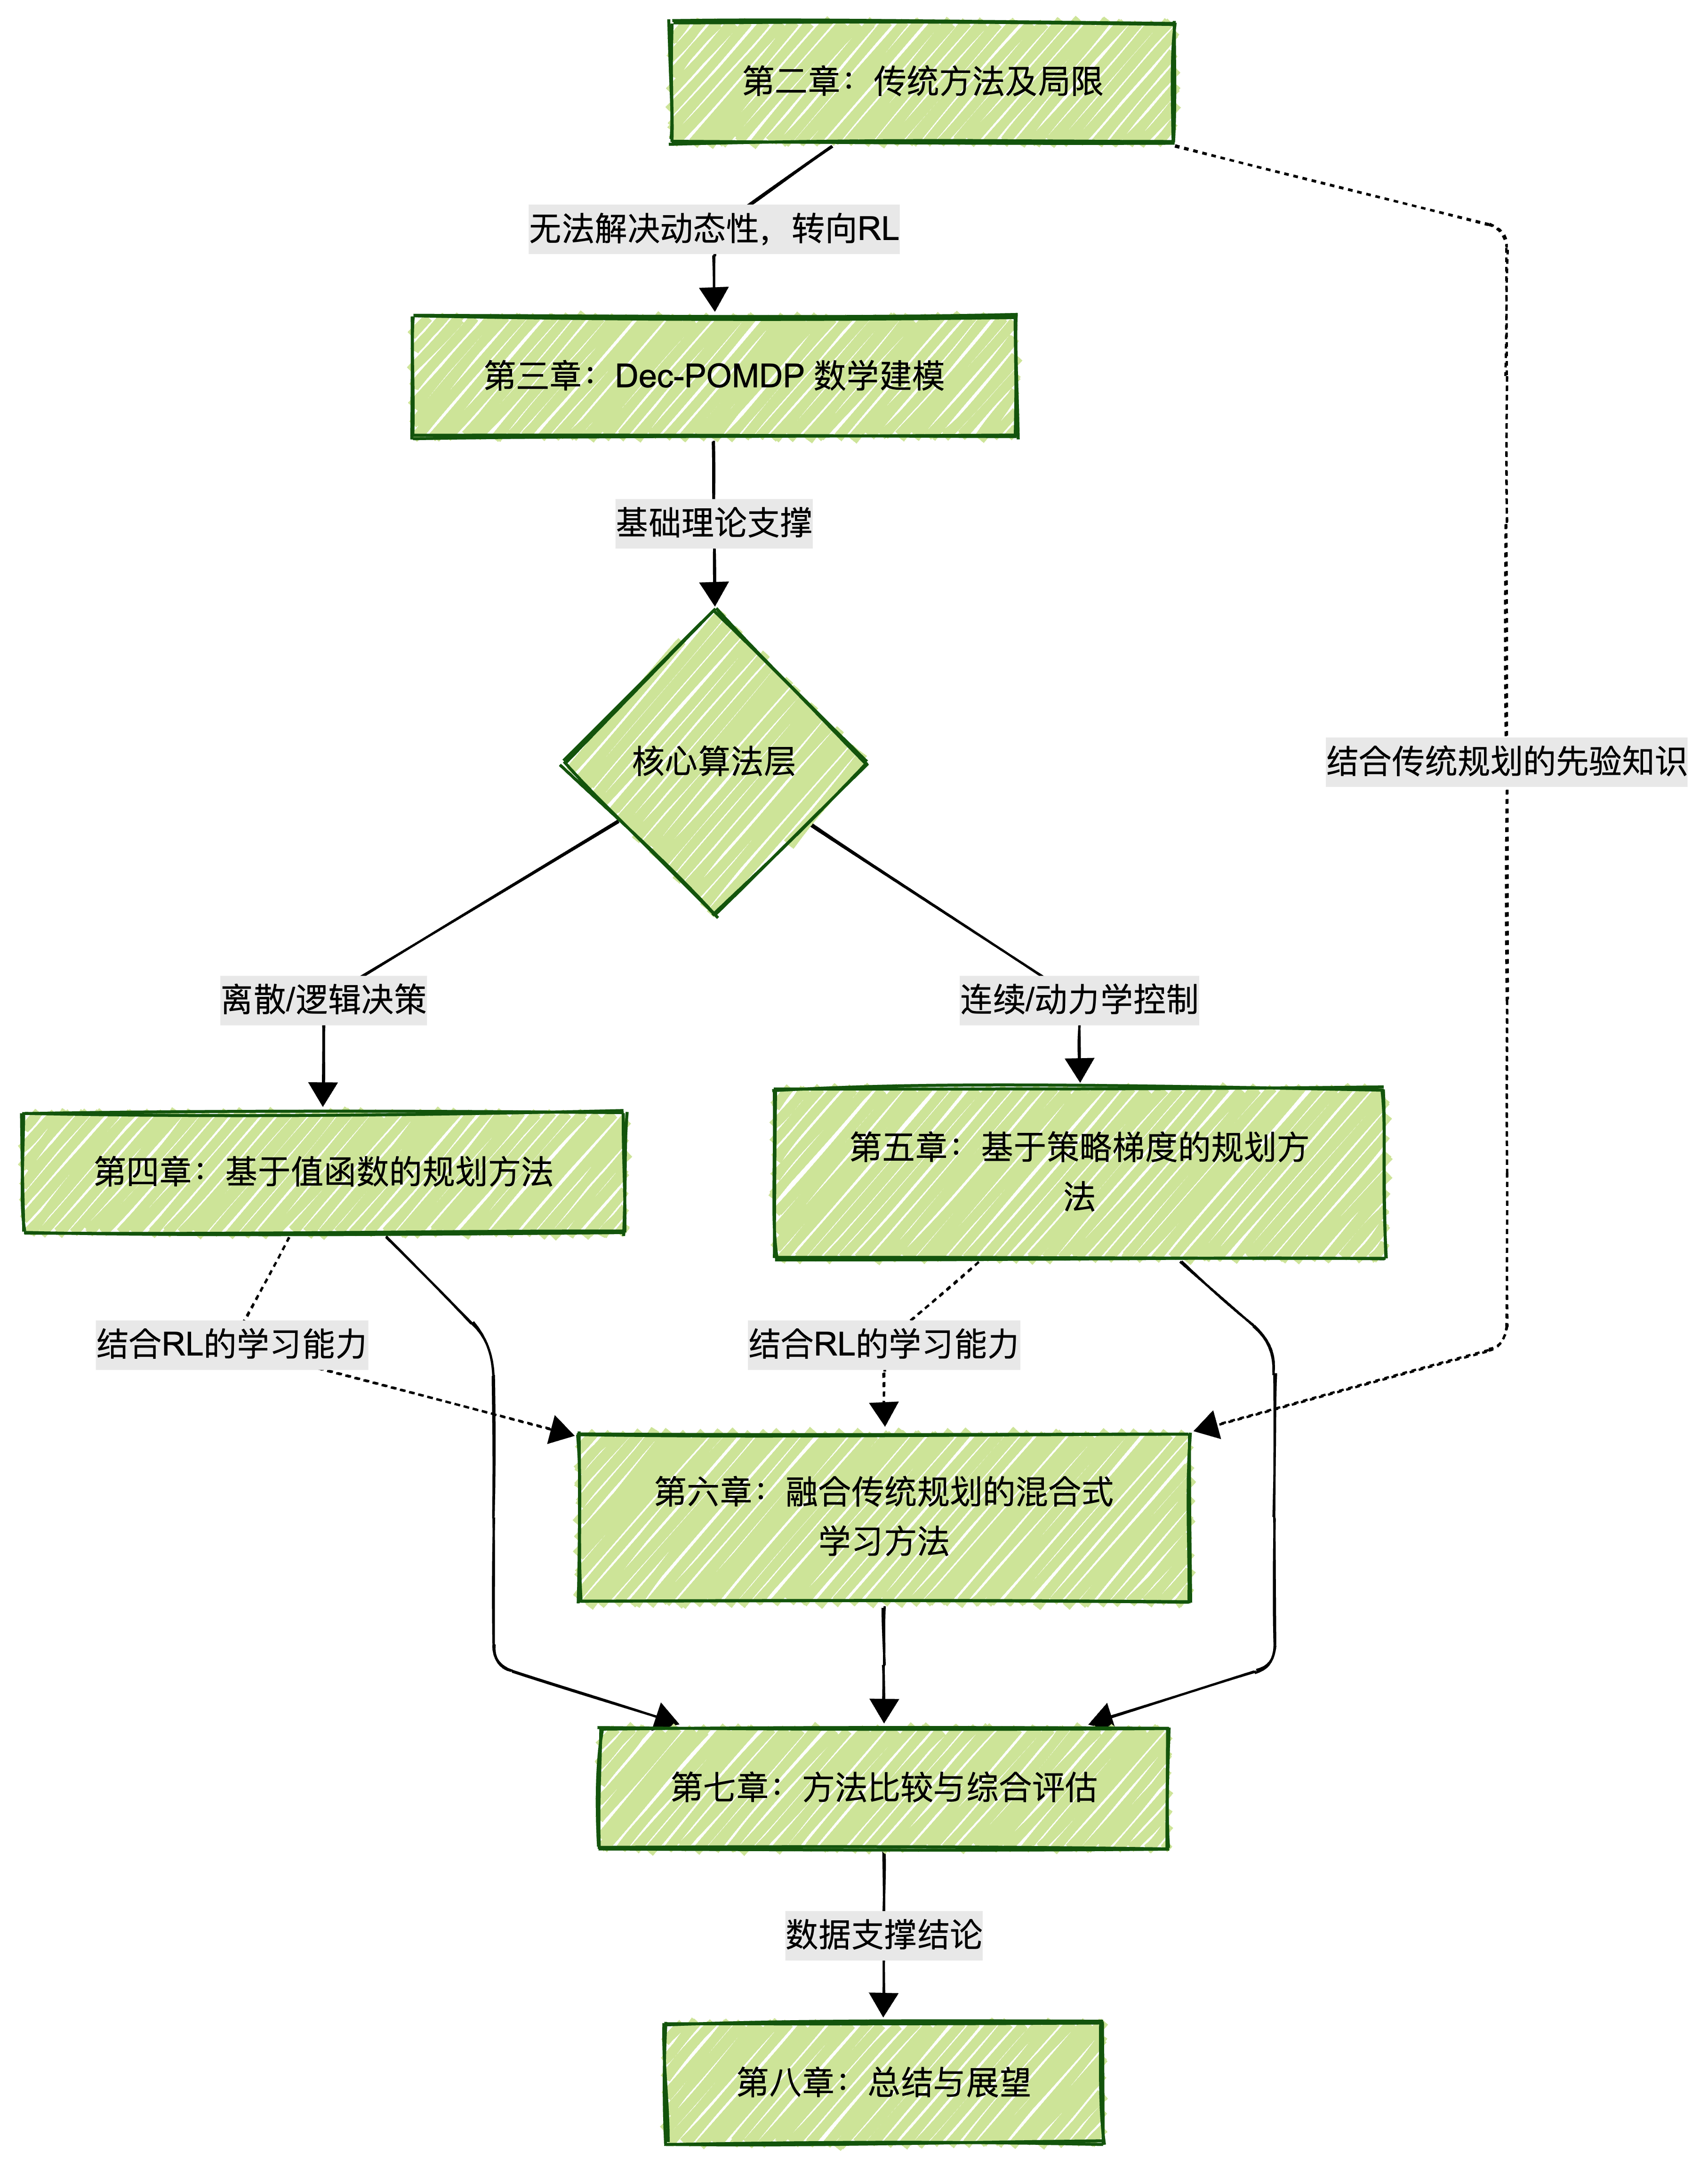
\includegraphics[width=1\textwidth]{figures/outline.png}
    \caption{\textbf{本文研究框架与章节组织结构图}}
    \label{fig:outline}
\end{figure}

\section{传统MAPF方法及其局限性}

多智能体路径规划（Multi-Agent Path Finding, MAPF）旨在为一组智能体在给定的环境中寻找从各自起点到终点的无碰撞路径，同时优化全局的运行时间或移动成本。尽管Yu和LaValle早已证明在图上求解最优 MAPF 问题是NP-Hard的~\cite{yu2013structure}，但经过几十年的演进，学界已发展出一套成熟的算法体系。这些经典方法构成了当前协同规划领域的基石，也是理解新兴强化学习方法优势与不足的必要前提。

\subsection{经典算法回顾}

多智能体协同规划的算法根基在于单智能体路径搜索，其中A*算法因其完备性与最优性而被视为黄金标准。A*算法通过维护一个优先级队列，利用评估函数 $f(n) = g(n) + h(n)$ 来指引搜索方向，其中 $g(n)$ 代表从起点到当前节点的实际代价，$h(n)$ 代表到终点的启发式预估代价。在多智能体场景下，最朴素的扩展是将所有智能体的状态组合成一个联合状态空间，并在其上运行 A* 算法。然而，这种方法的搜索空间大小随智能体数量呈指数级增长（$b^{N}$，其中 $b$ 为分支因子，$N$ 为智能体数量），迅速导致维数灾难。为了解决这一问题，Silver等人提出的分层协作 A*（HCA*）以及随后的窗口分层协作 A*（WHCA*）尝试在时空维度上进行解耦搜索~\cite{silver2005cooperative}，即后续智能体将先前智能体的规划路径视为动态障碍物进行规避。尽管这种基于优先级的解耦方法极大地提升了计算速度，但它丧失了完备性，在狭窄环境或高密度场景下极易因贪婪策略而陷入死锁，无法找到理论上存在的解。

为了在避免状态空间爆炸的同时保留算法的最优性与完备性，基于冲突的搜索（Conflict-Based Search, CBS）算法应运而生，并成为了 MAPF 领域的一个重要里程碑。CBS 摒弃了在联合状态空间中进行搜索的传统思路，转而采用一种独特的双层搜索架构：上层维护一棵约束树,通过检测不同智能体路径间的时空冲突，例如智能体 A 和 B 在时间 $t$ 同时占据位置 $v$，来生成约束条件；下层则为每个智能体独立调用 A* 算法，在满足上层约束的前提下寻找最短路径。

这种方法成功将复杂的多智能体耦合问题分解为一系列受约束的单智能体路径规划问题，极大地提升了求解效率，特别是在障碍物稀疏的开阔环境中表现优异。然而，CBS的性能高度依赖于冲突的频次，在拥堵环境中，频繁的冲突会导致约束树规模呈指数级膨胀，退化为一种低效的穷举搜索。
与上述基于网格图的离散搜索算法不同，在连续空间的导航与避障任务中，基于速度障碍物的反应式算法占据了主导地位，其中最优倒数防撞（Optimal Reciprocal Collision Avoidance, ORCA）是最具代表性的算法。ORCA 将避障问题转化为速度空间中的线性规划问题，其核心假设在于互惠性，即每个智能体假设对方也会分担一半的避障责任。在每个控制周期，ORCA根据邻居的位置和速度计算出一个半平面约束集合，智能体在这些约束的交集中选择一个最接近期望速度的新速度矢量。

这种几何方法计算复杂度极低，通常仅为 $O(N)$，因此非常适合大规模群体（如数千个智能体）的实时模拟。Van Den Berg 等人证明了 ORCA 在保证无碰撞的前提下能生成平滑的运动轨迹~\cite{sharon2015conflict}。但作为一种局部反应式方法，ORCA 缺乏全局规划视野，在面对迷宫般的复杂静态障碍物或局部最小值时，容易陷入震荡或死锁，无法保证能到达全局目标点。

\subsection{传统方法的局限性小结}

尽管上述经典算法在结构化、静态的实验环境中表现优异，但在面对现代物流仓储、无人机集群等大规模、高动态应用时，其局限性日益凸显，首当其冲的便是可扩展性瓶颈。对于以 CBS 为代表的最优或有界次优算法，其计算复杂度在本质上受到NP-Hard问题的约束，面临着严峻的组合爆炸挑战。随着智能体数量 $N$ 的增加或环境障碍物密度的提升，状态空间或约束树的规模呈指数级增长。

Ma 等人的基准测试表明，在涉及数百个智能体的复杂迷宫中，CBS往往需要在几秒甚至几分钟内才能完成一次规划，这完全超出了实时系统的容忍极限~\cite{skrynnik2024learning, shi2024multi}。另一方面，以ORCA为代表的解耦方法虽然在计算速度上具备线性扩展优势，但其代价是牺牲了算法的完备性。在狭窄通道或高密度拥堵区域，局部贪婪的避障策略极易导致智能体之间形成对称性死锁或相互阻挡，使得系统在大规模场景下的任务成功率呈现断崖式下跌，这种计算效率与求解质量之间的零和博弈是传统方法难以逾越的鸿沟。

在鲁棒性层面，传统MAPF算法普遍采用感知、规划、执行的开环控制模式，这种模式对环境模型和执行精度的要求近乎苛刻。算法通常假设当前处于全知状态，且环境是静态已知的，规划出的时空轨迹是基于完美的运动学模型计算的。然而，在现实物理系统中，感知噪声、通信延迟以及执行机构的误差是不可避免的常态。

对于基于精确时空预约的算法，任何微小的执行偏差，例如智能体 A 晚到了 0.5 秒，都可能导致原本无冲突的全局计划失效，进而引发连锁反应式的碰撞风险或系统死锁。Hönig等人指出，为了应对这种不确定性，传统方法往往需要设置较大的安全缓冲，但这又反过来显著降低了空间利用率和系统的整体吞吐量~\cite{honig2018trajectory}。这种对精确模型的过度依赖，使得传统算法在面对部分可观测或存在动态干扰的真实世界时显得极度脆弱。
最后，传统方法在在线性与泛化能力上也存在显著短板，难以满足即时响应的需求。大多数经典 MAPF 算法本质上属于离线规划,即在移动前必须获取完整的全局地图信息并完成所有计算。这意味着它们难以应对环境拓扑结构发生突变的场景。一旦环境发生变化，传统系统通常需要冻结所有智能体进行全局重规划,这在高维系统中不仅计算代价高昂，还会导致系统运行的非连续性卡顿。更为关键的是，传统算法是基于固定规则设计的，缺乏从历史数据中学习的能力。无论是在相同的环境中运行多少次，算法每次面对相似的拥堵路口时都是从零开始搜索，无法像人类一样通过经验积累形成直觉式的拥堵规避或排队策略。这种无记忆的特性限制了系统在长期运行过程中的效率进化，也使得算法难以直接迁移到未曾见过的复杂新环境中。

\section{问题定义与分类框架}

\subsection{多智能体强化学习}
强化学习（Reinforcement Learning, RL）作为机器学习的一个核心分支，通过智能体与环境的交互试错机制来学习最优策略，旨在最大化长期的累积奖励。与监督学习依赖标记数据不同，强化学习关注的是如何在未知环境中通过动作序列获得延迟反馈。在多智能体路径规划（MAPF）领域，引入强化学习使得智能体能够摆脱对精确环境模型的依赖，通过高维感知输入直接决策，从而具备处理动态障碍物和复杂交互的能力。本章将首先建立多智能体协同规划的数学模型，随后分析现实场景中的关键约束，最后构建主流算法的分类体系框架，为后续章节的深度分析确立理论基准。

\subsection{Multi-Agent Dec-POMDP建模}

\begin{figure}[htbp]
    \centering
    % 请在 Google Images 搜索 "Dec-POMDP diagram Oliehoek" 下载图片
    % 并命名为 dec_pomdp_model.png 放入 figures 文件夹
    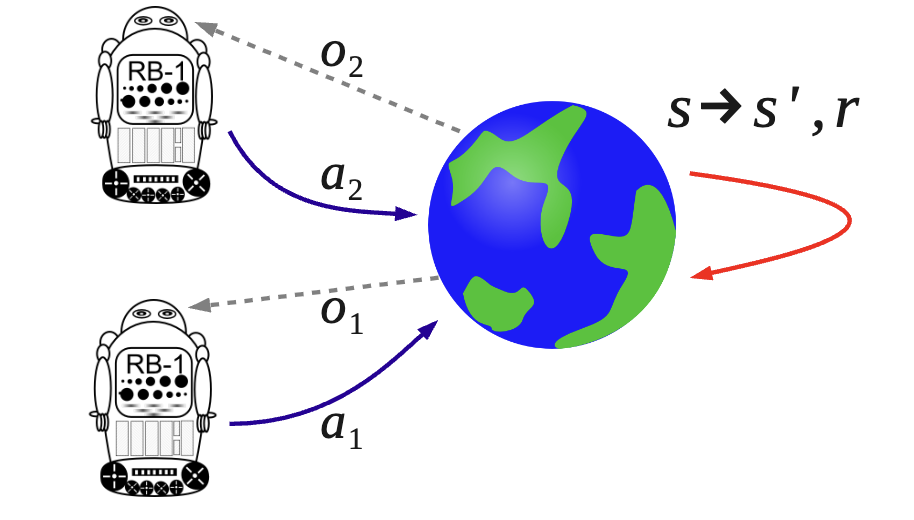
\includegraphics[width=0.7\textwidth]{figures/dec_pomdp_model.png}
    
    \caption{\textbf{Dec-POMDP 模型交互示意图}。该模型描述了 $N$ 个智能体与环境的离散时间交互过程。在每个时间步，环境处于真实状态 $s$，每个智能体 $i$ 仅能获得局部观测 $o_i$ 并获得局部奖励 $r_i$，随后根据自身策略 $\pi_i$ 独立选择动作 $a_i$。所有智能体的联合动作 $\boldsymbol{a}$ 共同决定了环境的状态转移 $P(s'|s,\boldsymbol{a})$ 和全局奖励分布。}
    % ~\cite{oliehoek2016concise}
    \label{fig:dec_pomdp_model}
\end{figure}

在多智能体路径规划任务中，由于每个智能体通常只能通过机载传感器（如激光雷达、深度相机）感知局部环境，且多个智能体的同时动作会导致环境状态转移的非平稳性，因此，去中心化部分可观测马尔可夫决策过程（Decentralized Partially Observable Markov Decision Process, Dec-POMDP）被公认为是描述此类问题的最通用且严谨的数学框架~\cite{oliehoek2016concise}。如图\figref{fig:dec_pomdp_model}所示，一个标准的 Dec-POMDP 模型可以由一个八元组 $\mathcal{M} = \langle \mathcal{I}, \mathcal{S}, \{\mathcal{A}_i\}, \mathcal{P}, \{\mathcal{R}_i\}, \{\Omega_i\}, \mathcal{O}, \gamma \rangle$ 来定义。其中，$\mathcal{I} = \{1, \dots, N\}$ 表示系统中 $N$ 个智能体的集合；$\mathcal{S}$ 表示环境的全局状态空间，它包含了所有智能体的位置、速度、姿态以及环境中的静态与动态障碍物分布信息。在每一个离散时间步 $t$，每个智能体 $i \in \mathcal{I}$ 根据其自身的策略选择一个动作 $a_i \in \mathcal{A}_i$，所有智能体的动作共同构成了联合动作向量 $\boldsymbol{a} = \{a_1, \dots, a_N\} \in \mathcal{A}$。环境的状态转移函数 $\mathcal{P}: \mathcal{S} \times \mathcal{A} \to \Delta(\mathcal{S})$ 定义了系统动力学，即在当前全局状态 $s$ 下执行联合动作 $\boldsymbol{a}$ 后，环境转移到下一状态 $s'$ 的概率分布 $P(s'|s, \boldsymbol{a})$。

与完全可观测的马尔可夫决策过程（MDP）显著不同的是，在 Dec-POMDP 设定下，智能体无法直接获取全局状态 $s$，而是必须依赖观测函数$\mathcal{O}(o_i|s, a_i)$ 来接收局部观测值 $o_i \in \Omega_i$。在路径规划的语境中，$\Omega_i$ 通常对应于传感器的视场角或通信范围内的拓扑信息，这意味着智能体必须在信息不完备的情况下进行决策。关于奖励函数的设计，对于完全合作型的协同规划任务，通常设定所有智能体共享一个全局奖励函数，即 $\mathcal{R}_1 = \dots = \mathcal{R}_N = R(s, \boldsymbol{a})$。这种共享奖励机制（如团队到达目标的总时间负值或无碰撞运行的奖励）旨在消除个体间的利益冲突，确立共同的优化目标。然而，在某些大规模稀疏奖励场景中，为了加速训练收敛，也会引入个体化的势能奖励作为辅助，但其核心目标始终是最大化团队效用~\cite{littman1994markov}。
最终，基于 Dec-POMDP 的协同路径规划问题的优化目标是寻找一个联合策略 $\boldsymbol{\pi} = \{\pi_1, \dots, \pi_N\}$，其中 $\pi_i$ 是智能体 $i$ 将其历史观测序列映射到动作空间的策略函数。该联合策略旨在最大化无限时域内的折扣累积期望回报 $J(\boldsymbol{\pi}) = \mathbb{E}_{\tau \sim \boldsymbol{\pi}} [\sum_{t=0}^{\infty} \gamma^t R(s_t, \boldsymbol{a}_t)]$，其中 $\gamma \in [0, 1)$ 是折扣因子，用于平衡即时避障需求与长远路径规划目标之间的权重。这一数学形式化不仅涵盖了智能体自身的运动学约束，也通过联合状态转移概率 $\mathcal{P}$ 隐式地包含了智能体间的物理交互与碰撞约束，为后续引入深度强化学习算法进行端到端的策略求解提供了标准的理论接口~\cite{sutton2018reinforcement}。

\subsection{关键约束与环境特性}

在将理论模型应用于实际物理系统时，必须充分考虑环境施加的硬性约束与特性，其中通信约束与感知不确定性是最为关键的两个现实因素。通信是多智能体协作的基础，但在真实场景中，如无人机集群或仓储机器人，通信带宽有限且存在延迟，甚至可能面临完全中断的风险。因此，算法设计必须在全通信与无通信之间寻找平衡，例如采用基于注意力机制的通信协议来筛选关键信息，或者设计连通性保持约束，确保智能体在移动过程中始终处于通信拓扑的连通分量内。若忽略通信约束，完全依赖中心化指令，一旦网络波动，整个集群的路径规划将面临瘫痪风险。
感知的局部性与不确定性则是另一个核心挑战。智能体的传感器不仅存在测量噪声，还会受到遮挡的影响，导致观测到的环境信息是不完整甚至是有误的。这种部分可观测性不仅使得智能体难以准确推断自身与其他智能体的相对位置，还可能导致非平稳性问题的加剧，即从单个智能体的视角看，由于其他智能体的策略在不断变化，环境的状态转移规律显得不稳定。为了应对这一特性，通常需要在策略网络中引入循环神经网络（RNN）或长短期记忆网络（LSTM）来整合历史观测信息，从而对隐状态进行推断，或者利用贝叶斯滤波等技术来构建对动态环境的置信度地图。

\subsection{主流算法范式与分类架构}

\subsubsection{主流算法范式}

在多智能体强化学习（MARL）解决协同路径规划（MAPF）问题的进程中，如何平衡训练阶段的全局信息利用与执行阶段的分布式通信约束，始终是算法设计的核心矛盾。为此，集中式训练-分布式执行（Centralized Training with Decentralized Execution, CTDE） 架构已成为当前最具统治力的通用范式。该架构巧妙地打破了信息壁垒：在训练阶段，算法允许访问全局状态 $s$、其他智能体的动作 $\boldsymbol{a}_{-i}$ 甚至其内部奖励函数，以此来缓解由于其他智能体策略变化而导致的环境非平稳性问题；而在测试与实际部署阶段，每个智能体 $i$ 仅需依赖自身的局部策略网络 $\pi_i(a_i|o_i)$，根据局部观测 $o_i$ 做出决策。最新研究表明，结合 Transformer 或图神经网络（GNN）的 CTDE 架构不仅保留了中心化方法在策略优化上的稳定性，更能有效处理大规模变长输入，满足了物理集群在去中心化部署时对通信带宽和计算效率的严苛要求~\cite{skrynnik2024learning, wang2023scrimp}。

在 CTDE 架构的具体实现中，基于 Actor-Critic 的方法 占据了重要地位，特别是在连续控制任务中。虽然经典的 MADDPG 奠定了基础，但近期的研究更倾向于结合安全约束与高效通信机制。现代变体通常为每个智能体维护一个能够感知邻居意图的 Critic 网络，利用注意力机制动态聚合全局信息，从而准确评估当前联合动作在复杂动态交互中的优劣。例如，针对无信号灯路口通行或无人机编队飞行，基于 PPO的多智能体变体（MAPPO）通过引入控制障碍函数或安全层，使得智能体不仅能显式学习到协作策略，还能在“试错”过程中保证系统的安全性与鲁棒性~\cite{yu2023surprising, gu2023safe}。

针对离散动作空间的协同规划任务，比如网格地图上的大规模仓储机器人调度，价值分解范式提供了另一种高效的思路。这类方法旨在解决合作博弈中的信贷分配难题。虽然早期的 VDN 和 QMIX 奠定了基础，但近年来的工作，如 QPLEX, QTRAN++ 以及基于 Transformer 的变体，致力于突破“单调性约束”对策略表达能力的限制。最新的研究倾向于在混合网络中引入时空图结构，利用 Transformer 的全局感受野来动态分配权重，从而在不需要显式单调假设的情况下，也能精确地将全局奖励 $Q_{tot}$ 分解为个体的局部 $Q_i$。这种改进使得算法在处理长视距规划和终身学习任务时，能够更敏锐地捕捉到瓶颈区域的死锁风险，并涌现出更复杂的交替通行行为~\cite{shao2024transformer, li2024scaling}。

\subsubsection{分类框架}

构建一个科学、全面的分类框架是理解多智能体路径规划技术演进路线的前提。本文基于最新的研究进展，从环境特性、控制结构及算法机理三个维度进行分类。

首先，环境特性是决定算法适用边界的最底层维度。依据环境的时空属性，场景可被划分为静态结构化与动态非结构化环境。经典的 MAPF 研究多聚焦于静态栅格地图，但在工业 4.0 背景下，研究重心正向动态且非结构化的连续空间转移（如人机共存的柔性车间）。此外，环境的随机性建模也至关重要，最新的算法倾向于在部分可观测马尔可夫决策过程（Dec-POMDP）框架下，引入域随机化或扩散模型来处理传感器噪声及执行器误差，以增强 Sim-to-Real 的迁移能力~\cite{zhao2024sim2real}。

其次，信息交互与控制结构 决定了系统的决策模式。除了传统的集中式和分布式架构外，当前的分类更关注通信机制的引入方式。现代 CTDE 架构通常被进一步细分为无通信 CTDE与基于通信的学习。前者仅利用隐式意图推断，而后者允许智能体在执行阶段通过受限带宽交换压缩的嵌入向量或图消息。研究表明，在极度拥堵或视距受限的场景下，引入显式的选择性通信机制能显著降低死锁率~\cite{xiao2023multi}。

最后，依据 算法范式的内在机理，现有的解决方案可被归纳为传统规划、在线/离线 RL 以及混合规划-学习四类。
\begin{itemize}
    \item \textbf{传统规划方法}：基于启发式搜索，近期工作重点在于通过大邻域搜索（LNS）提升其在大规模场景下的实时性~\cite{li2023lacam, huang2023anytime}。
    \item \textbf{在线强化学习}：通过实时交互更新策略，是解决异构智能体协同的主流方向，但面临样本效率挑战。
    \item \textbf{离线强化学习}：致力于从历史数据集（如人类专家驾驶数据）中学习保守策略，避免在线探索风险，是自动驾驶领域的探索热点。
    \item \textbf{混合规划-学习}：这是近年来的突破点，试图结合传统算法的长时程规划能力与 RL 的局部反应能力。例如，利用学习到的启发式函数加速 A* 搜索，或者利用构建好的路线图引导 RL 智能体穿越狭窄通道~\cite{okumura2024ctr}，从而实现了安全性与学习效率的双重提升。
\end{itemize}

\subsection{本文采用的综述分类框架}

基于上述分析，本文后续章节将采用一种以算法架构演进为主线，辅以应用场景特性的综合分类框架进行详细综述。具体而言，我们将重点聚焦于 CTDE 架构下的两大分支，基于价值分解的方法与基于Actor-Critic的方法，深入探讨它们在解决路径死锁与大规模协同时的内在机制。同时，为了突出现实意义，我们单独划分出一个类别来讨论混合规划与引导式学习，这类方法通过利用传统专家的演示数据或残差学习机制，有效解决了纯RL方法冷启动困难与安全性无法保证的问题。该分类框架旨在从理论深度与应用广度两个维度，清晰地呈现多智能体协同路径规划领域的技术脉络与前沿动态，不仅关注算法性能的指标提升，更关注其在处理通信受限、局部观测及动态干扰等真实约束下的适应能力。

\section{基于值函数的规划方法}

在多智能体强化学习（MARL）解决协同路径规划（MAPF）问题的进程中，基于值函数（Value-Based）的方法占据了主导地位。这类方法的核心思想是通过拟合一个价值函数来评估状态-动作对的优劣，进而通过贪婪策略选取最优路径。然而，直接将单智能体 Q-Learning 扩展到多智能体系统会面临环境非平稳性问题，而直接学习联合动作的 Q 值又会遭遇维数灾难。为了解决这一矛盾，集中训练–分散执行（CTDE）架构下的值分解方法应运而生，它成为了连接全局最优性与局部执行效率的关键桥梁。

\subsection{集中训练–分散执行的值分解方法}

值分解方法的核心假设在于，全局的联合价值函数 $Q_{tot}$ 可以被分解为所有智能体局部价值函数 $Q_i$ 的某种函数组合。这种架构在训练阶段允许利用全局状态信息来优化 $Q_{tot}$，从而隐式地指导局部 $Q_i$ 的更新；而在执行阶段，每个智能体仅需依据自身的局部观测 $o_i$ 和局部网络 $Q_i$ 进行贪婪决策，即可保证系统的整体协同性能。这一机制巧妙地解决了多智能体系统中的信用分配，即在复杂的动态交互中，准确判定是哪一个智能体的具体动作导致了最终的碰撞或成功到达~\cite{skrynnik2024learning}。

\subsubsection{VDN、QMIX 及其现代变体在路径规划中的实践}

作为值分解领域的奠基性工作，价值分解网络（VDN）提出了一种基于加法假设的简明架构，即假设 $Q_{tot}(\boldsymbol{\tau}, \boldsymbol{u}) = \sum_{i=1}^{n} Q_i(\tau_i, u_i)$。在多机器人路径规划的现代视角下，这种线性求和暗示了团队的总体收益等于个体收益的总和。最新的大规模仓储调度研究表明，在稀疏环境或同构机器人集群中，VDN 架构依然具备极高的样本效率，能够促使个体为了最大化团队总分而主动寻找目标。然而，其线性约束限制了对复杂博弈的表达能力，例如在“窄门”场景下，某个智能体必须做出较大的局部牺牲（如长时间等待）以换取全局最优，简单的加法难以精确建模这种非线性的收益权衡~\cite{li2024scaling}。

\begin{figure}[htbp]
    \centering
    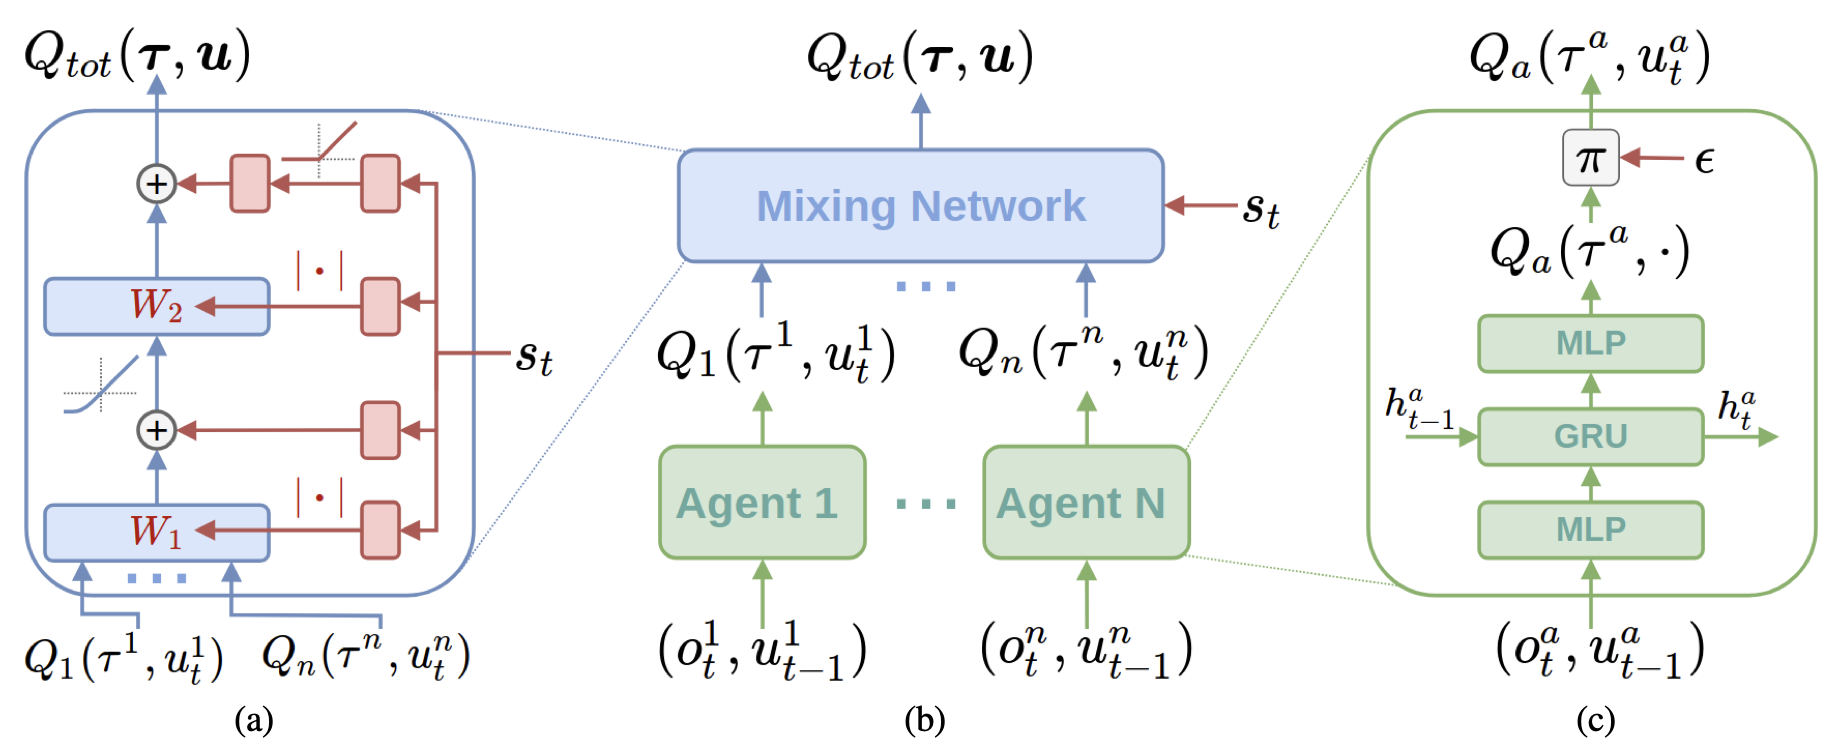
\includegraphics[width=0.9\textwidth]{figures/qmix_arch.png}
    \caption{\textbf{QMIX 算法架构示意图}。(a) 混合网络结构。红色部分为生成混合网络层权重与偏置的超网络（蓝色部分所示）;(b) QMIX整体架构;(c) 智能体网络结构。超网络利用全局状态 $s$ 动态生成混合网络的非负权重，从而在保证全局价值 $Q_{tot}$ 与局部价值 $Q_i$ 之间单调性约束的同时，实现对复杂环境状态的非线性建模。}
    \label{fig:qmix_arch}
\end{figure}

为了突破线性局限，基于 QMIX的混合网络架构成为了当前 MAPF 领域的基准。QMIX 引入了一个由全局状态 $s$ 生成权重的超网络，如图\figref{fig:qmix_arch}，将 $Q_{tot}$ 建模为局部 $Q_i$ 的非线性单调组合。近期的研究进一步将这一思想与 Transformer 技术结合，利用注意力机制动态调整混合网络的权重。这种机制使得算法能够敏锐地感知环境中的拓扑结构变化：在空旷区域，混合网络退化为近似线性组合以加速收敛；而在瓶颈区域，网络能够自动赋予关键智能体（如处于死锁节点的机器人）更高的权重。实验数据显示，在包含数百个智能体的终身路径规划任务中，这种结合了状态感知与非线性分解的策略，能够显著降低死锁率并提升系统的整体吞吐量，展现出超越传统启发式算法的鲁棒性~\cite{shao2024transformer, zhang2023heterogeneous}。

\subsubsection{单调值分解与可扩展性分析}

值分解方法之所以能够实现分散执行且保证联合策略的一致性，其理论根基在于个体全局最大化（Individual-Global-Max, IGM）原则~\cite{son2019qtran}。该原则要求： 
\begin{align}
    \operatorname{argmax}_{\mathbf{u}} Q_{\text{tot}}(\boldsymbol{\tau}, \mathbf{u}) = \begin{pmatrix} 
        \operatorname{argmax}_{u_1} Q_1(\tau_1, u_1), & 
        \dots, & 
        \operatorname{argmax}_{u_n} Q_n(\tau_n, u_n) 
    \end{pmatrix}
\end{align}
即联合动作的最优解等价于所有个体动作最优解的集合。为了满足这一原则，QMIX 对混合网络施加了严格的单调性约束，即要求全局价值 $Q_{tot}$ 关于每个局部价值 $Q_i$ 的偏导数非负（$\frac{\partial Q_{tot}}{\partial Q_i} \ge 0$）。这一数学性质确保了只要某个智能体提升了其自身的局部 $Q_i$ 值，全局的 $Q_{tot}$ 也会随之非减。在路径规划的语境下，这意味着个体层面的局部优化通常会对集体目标产生正面或中性的贡献，这与大多数无恶意的协作导航任务相吻合。

然而，单调性约束在带来计算便利的同时，也限制了函数逼近器的表达能力，构成了此类方法在复杂场景下的主要局限。在某些极端的路径规划博弈中，最优策略可能需要特定的非单调配合，比如，只有当智能体 A 执行动作 $\alpha$ 且智能体 B 执行动作 $\beta$ 时奖励极高，而单独执行任一动作奖励极低甚至为负，QMIX 往往难以收敛到这类策略。尽管后续出现的 QPLEX 等算法试图通过双层混合网络架构来放宽这一约束以实现完全表达能力~\cite{wang2020qplex}，但在大规模智能体（如 $N > 100$）的扩展性分析中，QMIX 依然表现出了较好的平衡性。相比于独立 Q 学习（IQL）的无法收敛和中心化 Q 学习的指数级爆炸，QMIX 的计算复杂度主要取决于混合网络的规模，其随智能体数量呈线性或轻微的超线性增长。这使得基于单调值分解的方法成为目前在成百上千个机器人的大规模集群调度中，极少数具备落地可能性的强化学习范式之一，尤其是在结合了课程学习或参数共享技术后，其可扩展性得到了进一步验证\cite{hu2020voronoi}。

\subsection{时空依赖与交互拓扑建模}

在多智能体协同路径规划的实际部署中，智能体往往面临着比理论模型更为严苛的感知约束，即无法获取全局状态且感知范围受限。这种部分可观测性使得环境对于个体而言呈现非马尔可夫特性，单一时刻的观测无法完全推断出周围动态障碍物的速度矢量或意图。同时，智能体之间的交互关系并非静态的网格邻接，而是随着相对距离和运动态势实时变化的动态拓扑。因此，为了构建高效的策略网络，必须引入能够处理时间序列依赖和空间拓扑关系的深度神经网络架构，即在时间维度上利用循环神经网络进行记忆整合，在空间维度上利用图神经网络进行交互推理。

\subsubsection{局部观测下的时序记忆处理}

针对部分可观测马尔可夫决策过程（POMDP）中的状态推断难题，引入循环神经网络（RNN）及其变体长短期记忆网络（LSTM）或门控循环单元（GRU）已成为处理时序依赖的标准范式。在经典的多智能体路径规划算法中，如 Everett 等人提出的 GA3C-CADR~\cite{everett2018motion}，智能体不再仅根据当前的快照观测进行决策，而是维护一个内部的隐状态向量，该向量通过 LSTM 单元不断聚合历史观测信息。这种机制使得智能体能够在记忆中编码周围邻居的运动趋势，从而有效地推断出动态障碍物的速度和加速度，甚至在发生短暂遮挡时仍能保持对目标位置的估计。Hausknecht 等人最早提出的深度循环 Q 网络（DRQN）~\cite{hausknecht2015deep} 证明了，在部分可观测环境下，利用 LSTM 整合历史信息可以显著提升策略的鲁棒性。在密集人群或高动态仓储环境中，基于 GRU 的策略网络能够有效识别出复杂的运动模式，比如对方正在进行绕行或紧急避让，从而避免了仅凭单帧观测导致的短视决策和路径震荡，显著提升了轨迹的平滑度与安全性。

\subsubsection{图卷积/图注意力刻画多智能体交互}

虽然卷积神经网络（CNN）在处理固定网格地图方面表现优异，但其固定的输入尺寸和对欧几里得结构的依赖，使其难以有效建模多智能体之间数量可变且无序的交互关系。为了解决这一问题，图神经网络（GNN）被引入到 MAPF 领域，将每个智能体建模为图中的节点，智能体之间的通信或感知关系建模为边，从而构建出一个动态的交互图。Jiang 等人 ~\cite{jiang2018graph} 率先提出了基于图卷积强化学习的多智能体控制框架，通过在图结构上进行消息传递，使得智能体能够感知到其 $k$ 阶邻域内的状态信息。更进一步，考虑到在复杂的交通路口或狭窄通道中，不同邻居对当前智能体决策的影响权重截然不同，例如，正前方的障碍物威胁远大于后方的队友，Li 等人 ~\cite{li2020graph} 将图注意力网络（GAT）引入路径规划，利用注意力机制动态计算邻居节点的重要性权重。这种方法赋予了智能体“有侧重”的感知能力，使其能够在数以百计的邻居中自动筛选出最具威胁或最需要协作的关键对象，从而在保证计算效率的同时实现了精细化的交互建模。

\subsubsection{大规模编队中的时空联合表示}

在涉及成百上千个机器人的大规模编队或集群任务中，单纯的时间记忆或空间交互往往不足以支撑全局协同，必须构建时空联合表示。Sartoretti 等人提出的 PRIMAL 框架~\cite{sartoretti2019primal}是这一方向的典型代表，该框架设计了一种混合架构，首先利用卷积层提取局部地图的空间特征，随后通过 LSTM 层处理时间序列信息，最后结合模仿学习（Imitation Learning）在离散网格中实现了大规模的协同移动。更先进的方法开始探索时空图神经网络（ST-GNN），这种架构试图在图卷积操作中直接嵌入时间维度，或者交替堆叠 GNN 层与 RNN 层，以便同时捕获拓扑结构的演变和节点状态的动力学特征。通过这种深度的时空融合，智能体不仅能够理解当前的队形结构，还能预测未来的队形变化趋势，这对于维持大规模无人机编队的几何形状或在极度拥堵的自动化码头中实现无死锁的交通流控制至关重要。这种联合表示显著提升了算法在面对环境规模扩展时的泛化能力，使得在少量智能体环境下训练的策略能够直接迁移应用到大规模集群中。

\subsection{小结}

总体而言，基于值函数的多智能体强化学习方法，特别是结合了集中训练–分散执行（CTDE）架构的值分解算法，在离散空间的多智能体协同路径规划任务中取得了显著的成功。这类方法的主要优势在于其较高的样本效率，得益于经验回放机制,算法能够高效地利用历史数据进行离线策略更新，从而显著降低了与环境交互的训练成本。此外，通过显式的价值分解（如 VDN 和 QMIX），这类方法成功解决了多智能体系统中的信贷分配难题，能够清晰地量化个体行为对全局目标的贡献。在仓储物流、像素游戏及网格交通调度等离散动作空间（如上、下、左、右、停止）场景中，基于值函数的方法能高效收敛至确定性（或近似最优）策略，展现出卓越的工程稳定性与实用价值。

然而，当应用场景从简化的网格世界拓展到复杂的连续物理控制时，基于值函数的方法面临着严峻的动作空间维数灾难。DQN及其变体本质上是为了处理离散动作而设计的，若要将其应用于需要精确速度控制或加速度控制的移动机器人，通常需要对连续动作空间进行离散化处理。这种离散化不仅会导致控制精度的丢失，产生在极值间频繁切换的抖动轨迹，而且随着离散粒度的细化，动作空间的大小将呈指数级增长，导致寻找最大 Q 值的计算代价变得不可接受。尽管已有相关研究尝试在连续域内进行 Q 值拟合，但在高维的多智能体联合状态空间下，拟合函数的复杂度和训练的不稳定性依然是难以逾越的障碍。因此，在涉及无人机姿态控制或机械臂协同等对动作连续性要求极高的场景中，基于值函数的方法往往表现不如基于策略梯度的方法。

此外，模型表达能力的内在约束也是限制值分解方法泛化性能的关键因素。如前所述，为了满足 IGM 原则以实现去中心化执行，主流算法如 QMIX 强制施加了单调性约束。这种约束虽然保证了训练的可行性，但也限制了算法所能表示的联合价值函数的函数类范围。Mahajan 等人~\cite{mahajan2019maven}的研究指出，单调性约束使得算法难以学习到非单调的收益矩阵，而在复杂的协同路径规划任务中，这种非单调性并不罕见，比如，只有当两个智能体同时采取特定高风险动作时才能解锁通向目标的捷径，否则任何单方尝试都会导致极低的惩罚。在这种情况下，基于值函数的方法容易陷入次优的局部纳什均衡，缺乏有效的探索机制来跳出由于单调性假设带来的策略限制。这种对确定性策略的偏好也使得它们在需要随机策略来打破对称性死锁的场景中显得力不从心。

\section{基于策略梯度的规划方法}

随着多智能体系统在自动驾驶、无人机集群以及精密工业控制等领域的深入应用，环境的状态空间与动作空间呈现出高度的连续性特征。上一章讨论的基于值函数的方法（如 QMIX）虽然在离散决策层面表现优异，但在处理如车辆加速度、转向角或机械臂关节力矩等连续变量时，往往需要进行繁琐的离散化处理，这不仅会导致控制精度的损失，还可能引发维数灾难。为了克服这一瓶颈，基于策略梯度（Policy Gradient, PG）的方法通过直接参数化策略函数并在连续空间中搜索最优解，成为了解决复杂动力学约束下协同规划问题的关键技术路径。本章将详细探讨确定性与随机性策略梯度算法在多智能体路径规划中的演进脉络及其核心机制。

\subsection{确定性策略梯度与连续控制}

在单智能体连续控制领域，深度确定性策略梯度（Deep Deterministic Policy Gradient, DDPG）算法被视为是将 DQN 的成功经验迁移至连续动作空间的里程碑。DDPG 基于 Silver 等人提出的确定性策略梯度定理~\cite{silver2014deterministic}，采用 Actor-Critic 架构，其中 Actor 网络直接输出确定性的动作向量 $\mu(s|\theta^\mu)$，而 Critic 网络则通过逼近 $Q(s,a|\theta^Q)$ 来评估该动作的价值。然而，直接将 DDPG 简单复制到多智能体系统（即 Independent DDPG）在路径规划任务中表现极不稳定。这是因为在多智能体环境中，从单个智能体的视角来看，环境的状态转移不仅取决于其自身的动作，还取决于其他智能体的行为。随着所有智能体同时更新其策略，环境呈现出剧烈的非平稳性，导致 Critic 学习到的价值函数 $Q$ 实际上是一个随时间剧烈波动的目标，使得策略梯度的方向无法准确指引智能体实现协同避障。

\begin{figure}[htbp]
    \centering
    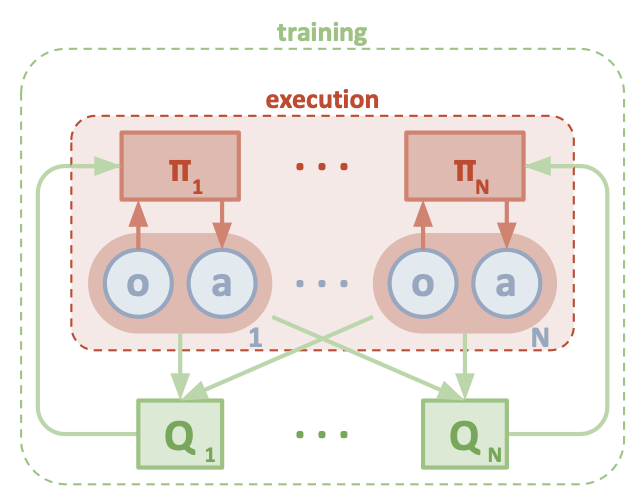
\includegraphics[width=0.55\textwidth]{figures/maddpg_framework.png}
    \caption{\textbf{MADDPG 集中训练-分散执行（CTDE）框架}。图中展示了算法的非对称信息结构：在训练阶段（Training），中心化的 Critic 网络利用所有智能体的观测与动作信息来评估策略价值；在执行阶段（Execution），分布式的 Actor 网络仅依赖局部观测进行决策}
    \label{fig:maddpg_framework}
\end{figure}

为了解决多智能体环境下的非平稳性挑战，Lowe 等人提出了多智能体深度确定性策略梯度（MADDPG）算法~\cite{lowe2017multi}，该算法成为了集中训练–分散执行（CTDE）范式在连续控制领域的奠基之作。MADDPG，如图\figref{fig:maddpg_framework}所示，的核心创新在于重新设计了 Critic 的输入结构：虽然每个智能体的 Actor 网络仍然仅依赖局部观测 $o_i$ 进行决策（这保证了执行阶段的分布式特性），但在训练阶段，每个智能体的 Critic 网络被增强为可以接收全局信息。具体而言，Critic 的输入不仅包含当前智能体的局部观测和动作，还包括了其他所有智能体的观测 $o_{-i}$ 和动作 $a_{-i}$（或全局状态 $s$）。这种全局感知的 Critic 实际上拟合的是联合动作价值函数 $Q_i^{\boldsymbol{\pi}}(\mathbf{x}, a_1, \dots, a_N)$。通过引入其他智能体的动作作为显式输入，Critic 能够将环境的动态变化“固定”下来，从而使得即便其他智能体的策略在不断更新，当前智能体也能准确评估在特定联合动作下的期望回报。这种机制成功地将一个非平稳的多智能体学习过程转化为一个对于 Critic 而言相对平稳的回归问题，从而保证了训练的收敛性。

在具体的协同路径规划与避碰应用中，MADDPG 展现出了显著优于传统离散方法的运动学平滑性。在处理自动驾驶车队或无人机编队的避障任务时，动作空间通常由线加速度和角速度组成。传统离散方法往往会导致非最优、抖动的轨迹，而 MADDPG 能够输出连续变化的控制量，生成符合动力学约束的平滑轨迹。例如，在狭窄通道的会车场景中，智能体不仅仅是简单地选择停止或前进，而是能够精细地调整转向角和速度，通过微小的横向偏移和速度协同来完成高效的相互绕行。研究表明，在包含物理惯性和摩擦力等复杂动力学特性的仿真环境中，MADDPG 能够学习到类似人类驾驶员的互惠性避让策略——即智能体 A 稍微向左偏转并减速，同时预期智能体B会做出相应的向右偏转，从而在不完全停车的情况下实现无碰撞通行~\cite{everett2018motion}。这种基于连续梯度的协同优化能力，使得MADDPG成为了解决高维、高动态且对控制精度有严格要求的多智能体规划任务的首选基准算法。

\subsection{随机性策略梯度与大规模协作}

尽管 MADDPG 在连续控制任务中展现了理论上的可行性，但在实际应用中，确定性策略往往容易陷入局部最优，且对超参数的选择极度敏感，这种脆弱性在智能体数量增加时表现得尤为明显。为了克服这一难题，基于随机策略的算法逐渐成为了大规模协同规划的主流范式，其中多智能体近端策略优化（Multi-Agent PPO, MAPPO）是最具代表性的算法。MAPPO 将单智能体领域表现最稳定的 PPO 算法扩展至CTDE架构，其核心机制在于引入了截断的目标函数，限制了每次策略更新的幅度，从而确保了训练过程的单调改进。Yu 等人~\cite{yu2022surprising}的实证研究表明，尽管MAPPO属于同策略算法，理论上的样本利用率低于异策略算法，但凭借其卓越的数值稳定性和对超参数的鲁棒性，它在星际争霸II等多智能体基准测试以及大规模无人机集群路径规划任务中，最终的收敛效果和成功率往往显著优于 MADDPG 和 QMIX。在处理大规模同构车队时，MAPPO 通常结合参数共享机制，即所有智能体共享同一个策略网络权重但输入各自的局部观测，这极大地压缩了参数空间，使得算法能够轻松扩展至控制数百甚至数千个智能体的协同运动，而不会遭遇维数灾难。

除了稳定性和可扩展性，如何在复杂的未知环境中保持高效的探索能力是路径规划的另一大挑战，软 Actor-Critic（Soft Actor-Critic, SAC）算法为此提供了优雅的解决方案。SAC 基于最大熵强化学习（Maximum Entropy RL）框架，其目标函数不仅最大化累积奖励，还试图最大化策略的熵。这一修正项鼓励智能体在学习过程中保持动作的多样性与随机性，避免在训练早期过早收敛到某一条单一的次优路径。在多智能体路径规划的语境下，SAC 的这种特性极具价值：当首选路径被动态障碍物意外阻断时，具有高熵特性的策略能够迅速切换到备选路径，表现出极强的抗干扰能力。Haarnoja 等人 ~\cite{haarnoja2018soft} 证明了 SAC 作为一种异策略算法，结合了重参数化技巧（Reparameterization Trick）和双 Q 网络机制，不仅在样本效率上远超 PPO，还能在连续空间中学习到多模态的驾驶策略（例如在路口既可以选择左侧绕行也可以选择右侧绕行），这种多样化的策略分布对于解决多智能体间的对称性死锁至关重要。

综上所述，从 MADDPG 到 MAPPO 再到 SAC 的演进，反映了多智能体规划算法在确定性与随机性、稳定性与效率之间的权衡与取舍。在实际的工程部署中，目前的趋势呈现出分化的态势：对于仿真环境稳定、对训练时间不敏感但追求极致大规模协同（如千机编队表演）的场景，MAPPO 凭借其简单可靠成为了首选基准；而对于数据获取昂贵、环境动态性极强且需要快速适应的实机机器人导航任务，基于 SAC 的异策略方法则因其极高的样本效率和探索能力而更受青睐。未来的研究方向正致力于融合两者的优势，例如在 MAPPO 框架中引入 SAC 的熵正则化项，或利用 PPO 的信任域约束来稳定 SAC 的训练过程，以期构建出兼具大规模扩展性与高效探索能力的通用型协同规划算法。

\subsection{结构化与分层策略增强}

尽管端到端的强化学习在局部反应式避障中表现卓越，但在面对具有长视距特征的大规模地图导航任务时，单纯依赖扁平化的策略网络往往难以为继。这是因为随着环境尺度的扩大，稀疏奖励问题变得极度尖锐——智能体可能在数千步的探索中都无法触及目标点，导致梯度更新停滞。为了打破这一瓶颈，分层强化学习（HRL）引入了时间抽象的概念，将复杂的长程导航任务分解为多层级的决策过程。典型的双层架构通常由上层策略（Manager）和下层策略（Worker）组成：上层策略不直接控制电机或速度，而是根据全局地图信息生成一系列短期的子目标；下层策略则以此子目标为导向，并在有限的时间窗口内输出具体的运动控制指令以抵达该子目标。Nachum等人~\cite{nachum2018data}提出的 HIRO 算法证明了这种架构的有效性，通过让上层策略在抽象的目标空间中进行规划，下层策略专注于解决局部的动力学控制与动态避障，系统能够有效地在迷宫般的复杂环境中实现跨越长距离的协同导航，避免了智能体在局部极小值处打转。

除了纯粹的学习型分层架构，工业界更倾向于采用结合传统全局规划和局部强化学习的混合范式，这种结构巧妙地结合了基于搜索算法的完备性与基于学习算法的适应性。在这类框架中，传统的图搜索算法（如 A*、Dijkstra 或 PRM）被用于在静态地图上快速生成一条几何上可行但可能不平滑的全局参考路径；随后，该路径被离散化为一系列密集的引导点输入给 RL 智能体。RL 智能体的任务不再是茫然地探索整个地图，而是学习如何在紧紧跟随这些引导点的同时，灵活地处理局部出现的动态障碍物或未知扰动。Faust 等人~\cite{faust2018prm} 提出的 PRM-RL 框架便是这一思路的经典实践，它利用概率路图（PRM）连接自由空间，通过 RL 学习点到点的导航策略，成功将长距离导航问题简化为一系列短程的导航任务链。这种混合方法通过大幅缩减状态空间的探索范围，在显著提升样本效率的同时，还从理论上为系统状态可达性提供了概率保障。这从根本上解决了纯强化学习方法因探索不充分导致的收敛失败或轨迹不可达等鲁棒性问题。

为了进一步提升系统在复杂交互环境下的安全性与训练效率，基于残差学习的结构化策略增强方法逐渐成为研究热点。与从零开始学习策略不同，残差强化学习假设智能体已配备了一个基础的传统控制器（如基于人工势场法 APF 或 ORCA 的控制器），该控制器虽然不是最优的，但能提供基本的避障能力。RL 策略网络的作用被重新定义为学习一个修正量，即最终输出动作 $a = a_{base} + \lambda a_{rl}$。这种架构使得智能体在训练初期就具备了基本的导航能力，避免了随机探索带来的危险碰撞。Silver等人~\cite{johannink2019residual}的研究表明，在多智能体协同场景中，利用RL学习残差可以有效地修正传统算法在死锁处理上的不足，例如在ORCA陷入震荡时，RL分支会输出一个额外的侧向推力来打破对称性。这种结构化设计融合了控制理论的稳定性与深度学习的灵活性，使得算法既能快速冷启动，又能在长期运行中不断进化出超越传统专家的复杂行为。

\subsection{讨论}

尽管基于策略梯度的方法（特别是 Actor-Critic 架构）成功地将多智能体路径规划拓展到了连续控制领域，并赋予了智能体处理复杂动力学约束的能力，但其训练过程的稳定性始终是学术界和工业界关注的核心痛点。与基于值函数的方法通过贝尔曼算子强制收敛不同，Actor-Critic 方法依赖于 Actor 网络与 Critic 网络之间的相互博弈与协同进化。Henderson 等人~\cite{henderson2018deep}的广泛实证研究指出，这种耦合结构极其脆弱：如果 Critic 网络在训练初期无法提供准确的价值估计，Actor 就会朝着错误的方向更新策略，而变差的策略又反过来导致 Critic 更加难以拟合，从而引发严重的性能震荡甚至策略坍塌。在多智能体场景下，这种不稳定性被进一步放大，因为任何一个智能体策略的微小波动都会改变全局的状态转移分布，导致其他智能体的学习目标发生偏移。因此，复现 MADDPG 或 MAPPO 等算法的性能往往需要精细的超参数调优以及特定的随机种子，这极大地增加了算法在实际工程项目中的调试成本与不可预测性。

样本效率低下是策略梯度方法面临的另一大瓶颈，尤其是在无法进行大规模并行仿真的物理机器人任务中。以 MAPPO 为代表的同策略算法，虽然理论收敛性较好，但其每一轮更新都需要丢弃旧的采样数据，导致为了习得一个简单的局部避障策略，往往需要与环境交互数百万次。即便是像 SAC 这样的异策略算法，尽管能够复用历史数据，但在高维连续空间中探索出一条稀疏奖励下的可行路径仍然如同大海捞针。为了缓解这一问题，当前的研究往往依赖于分布式强化学习架构，利用成百上千个 CPU 核心并行采集数据以暴力提升训练速度。然而，这种对算力的巨大需求限制了其在边缘计算设备或算力受限的嵌入式系统上的在线学习能力，迫使现有的解决方案大多停留在离线集中训练的阶段，难以实现真正的在线终身学习。

最后，从仿真环境到物理世界的迁移（Sim-to-Real Transfer）是策略梯度方法落地应用时必须跨越的鸿沟。在仿真器中，物理引擎通常是理想化的，缺乏现实世界中普遍存在的传感器噪声、执行器延迟、轮胎摩擦系数的不均匀分布以及复杂的空气动力学干扰。策略网络倾向于过拟合仿真环境的特定物理特性，甚至学会利用仿真器的数值积分误差来获得高分（例如产生高频振动来移动）。当这种策略直接部署到实体机器人上时，往往会表现出剧烈的抖动或完全失效。为了弥补这一差距，Tobin 等人~\cite{tobin2017domain}提出的域随机化技术成为了标准配置，通过在训练过程中随机扰动物理参数，迫使策略学习到对物理模型误差具有鲁棒性的行为特征。尽管如此，如何保证在具备安全约束的前提下，将基于连续控制的 RL 策略无缝部署到自动驾驶汽车或工业移动机器人等安全关键系统中，依然是一个尚未完全解决的开放性难题。

\section{融合传统规划的混合式学习方法}

在多智能体协同路径规划（MAPF）的实际演进中，纯粹的强化学习方法往往受限于低效的探索机制，特别是在迷宫般的复杂环境或极度稀疏的奖励设定下，智能体极易陷入局部最优或在训练初期长时间无法获得正向反馈。与此同时，基于搜索的传统算法虽然在大规模实时计算上存在瓶颈，但其在离线状态下能够提供理论上完备甚至最优的路径解。因此，融合传统算法理论保障与强化学习灵活适应性的混合学习范式，已成为突破现有性能瓶颈的关键方向。本章将系统阐述此类混合架构，涵盖从基于专家示教的模仿学习，到规划与学习形成深度闭环的系列方法。

\subsection{基于专家示范的模仿学习框架}

在强化学习的初期阶段，智能体通常采取随机漫步的方式探索环境，这种从零开始的学习方式在状态空间巨大的多智能体系统中表现得极度低效，被称为冷启动问题。为突破此困境，基于专家示范的模仿学习 框架被提出。其核心在于引入一个离线运行的中心化传统规划器作为专家，以生成高质量的 (状态， 动作) 示范序列。智能体通过对此专家数据进行监督学习，从而高效习得基础的避障与路径搜索规则。Sartoretti等人提出的PRIMAL~\cite{sartoretti2019primal}是这一领域的开创性工作。如图\figref{fig:primal_framework}所示，PRIMAL 采用了一种混合的训练目标函数，将模仿学习的交叉熵损失与强化学习（A3C 算法）的优势函数损失相结合。该方法的核心机制是融合集中式规划的专家知识与分布式强化学习。具体流程为：使用完备的集中式规划器 ODrM* 在随机地图上生成可解决智能体冲突的最优轨迹，作为专家数据；随后，在训练中为智能体引入一个模仿损失，强制其策略分布与专家动作对齐，从而在探索奖励的同时，高效模仿专家的避障与协同决策。

\begin{figure}[htbp]
    \centering

    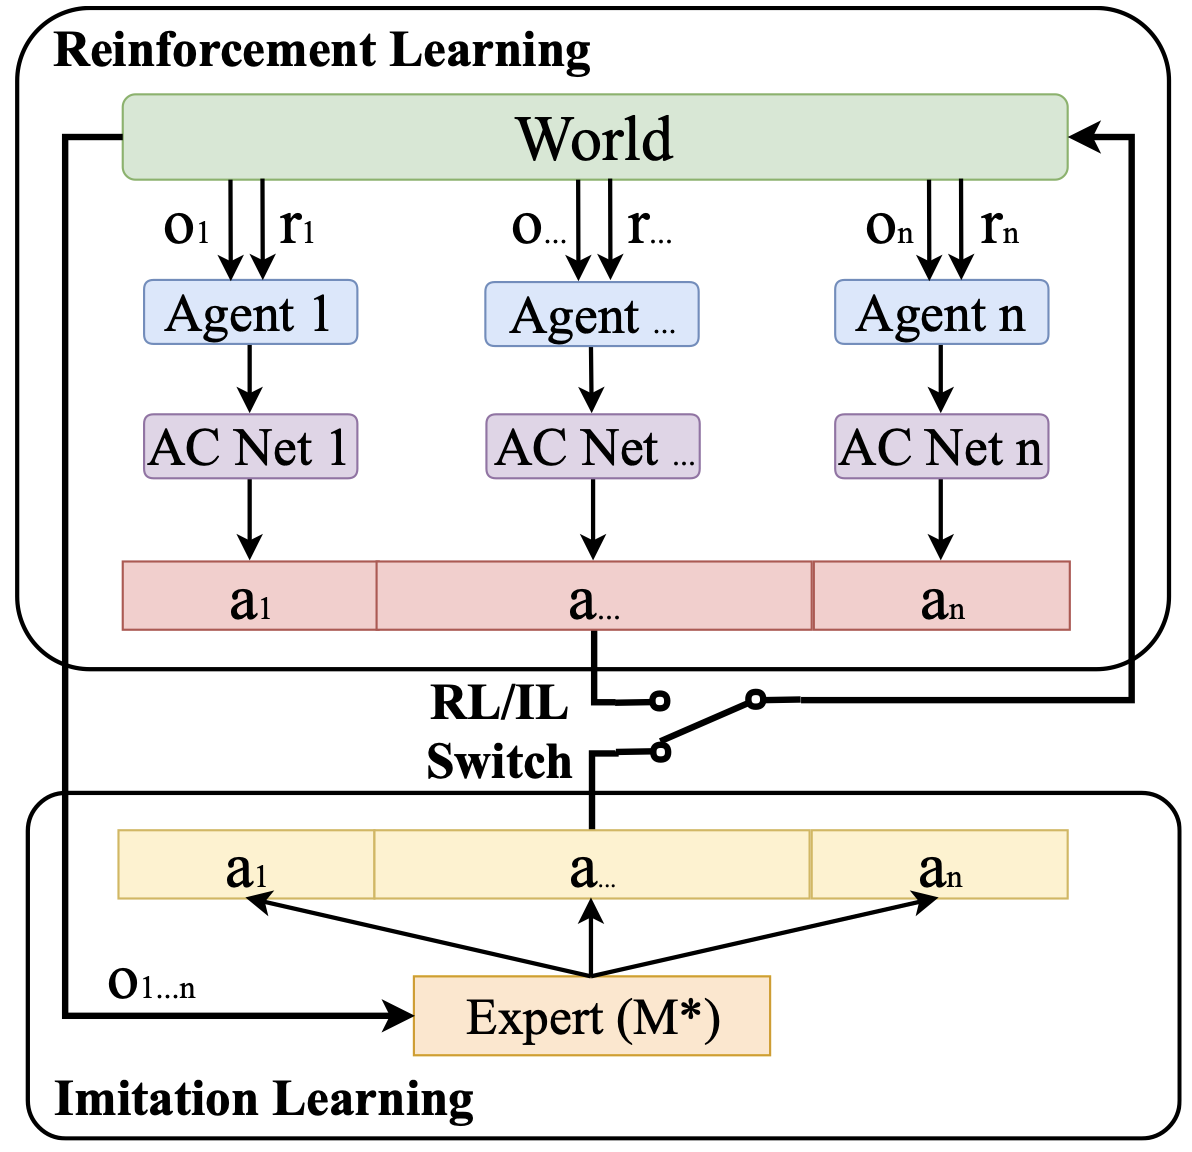
\includegraphics[width=0.5\textwidth]{figures/primal_flow.png}
    \caption{\textbf{图 6-1 PRIMAL 混合训练框架示意图}。系统采用双流训练机制：一方面利用传统专家规划器（Expert）生成的演示轨迹计算模仿学习损失（$L_{IL}$），加速策略冷启动；另一方面通过与环境交互计算强化学习损失（$L_{RL}$），提升策略在动态环境中的适应性。两者共同优化共享的神经网络参数。}
    
    \label{fig:primal_framework}
\end{figure}

这种混合训练机制不仅极大地加速了策略网络的收敛速度，还有效缓解了稀疏奖励带来的梯度消失问题。纯强化学习常受困于稀疏奖励问题，智能体需要大量低效试错才能获取有效反馈。引入专家示范则通过提供高质量的轨迹数据，为智能体注入了强大的行为先验。这使得智能体在训练初期就能学习到如目标导向移动和通道有序协作等关键行为模式，极大地加速了策略收敛，为学习鲁棒、高效的策略奠定了坚实基础。值得注意的是，PRIMAL 并非简单地进行行为克隆，因为单纯的克隆会导致分布偏移，即当智能体因误差偏离了专家轨迹后，由于从未见过该错误状态，往往无法纠正回正确的路径。PRIMAL 通过在训练后期逐渐降低模仿学习的权重，让 A3C 的强化学习机制占据主导，从而赋予智能体在专家未曾覆盖的复杂状态下进行自我探索和纠错的能力。这种策略使得最终习得的模型兼具了专家算法的规划合理性与 RL 算法的泛化鲁棒性，能够在未见过的地图和不同规模的团队中实现有效的去中心化协同。

随着研究的深入，针对 PRIMAL 框架在极度密集场景下死锁处理能力的不足，后续工作如 PRIMAL2~\cite{damani2021primal2}进一步细化了专家示范的作用机制。传统的 ODrM* 专家虽然能给出无冲突路径，但其决策往往依赖全局信息，直接强迫仅有局部观测的 RL 智能体去模仿基于全局信息的决策可能会产生认知失调。例如，专家算法可能会为了全局最优让一个智能体在空地上无故等待，而局部观测的智能体无法理解这一行为的动机。为了弥补这一信息鸿沟，改进的框架通常会在模仿学习阶段引入常规化约束，或者筛选出那些仅依赖局部信息即可解释的专家动作进行重点模仿。此外，通过构建课程学习机制，先让智能体模仿简单环境下的专家行为，再逐步过渡到模仿处理死锁和瓶颈的高级战术，这种分阶段的混合学习范式已成为解决大规模 MAPF 任务中“探索-利用”平衡难题的标准解决方案之一。

\subsection{规划–学习闭环一体化框架}

在模仿学习之外，另一种更为深度的混合策略是将强化学习模块直接嵌入到传统规划器的核心循环中，或者反之，将传统规划器作为强化学习的安全外壳。此闭环框架的本质，在于实现模型驱动规划与数据驱动学习的协同。它通过深度学习克服传统启发式函数的表征瓶颈与环境适应性不足，同时利用形式化约束保障神经网络策略的安全性底线，从而系统性地解决了效率、最优性与鲁棒性难以兼得的决策难题。

\subsubsection{“学习启发式”：RL 学习规划启发式或代价函数}

传统的基于搜索的 MAPF 算法极其依赖启发式函数（Heuristic Function, $h(n)$）的质量来引导搜索方向。在简单的空旷地图中，曼哈顿距离或欧几里得距离是足够有效的，但在涉及密集动态障碍物或复杂迷宫结构的环境中，这些静态启发式往往会产生极大的误导，导致搜索算法探索大量无效的状态节点。为了解决这一问题，研究者提出利用强化学习来训练一个参数化的价值函数 $V(s; \theta)$，并将其直接用作搜索算法中的启发式估计。Bhardwaj 等人 ~\cite{bhardwaj2017learning} 提出的学习启发式搜索框架证明了，通过 Q-Learning 或策略梯度训练出的价值网络能够捕捉到地图中的瓶颈、拥堵趋势以及智能体间的潜在冲突。通过将此神经网络作为启发式估计器集成到A框架中，我们实际上为搜索算法赋予了一个基于学习的决策组件。该组件能够融合全局趋势与局部观察，直接预测每个候选路径分支的远期代价与成功可能性。这使得A的搜索树能够被有效引导，专注于开发那些动态可行性最高的路径区域。这种方法保留了搜索算法的完备性和最优性框架，同时利用 RL 的泛化能力将搜索空间大幅剪枝，使得原本需要指数级时间求解的复杂协同问题可以在多项式时间内找到高质量解。此外，Gao 等人~\cite{gao2020g2rl}提出的 G2RL 框架进一步将这种思想扩展，该方法利用图神经网络（GNN）对系统全局拓扑进行编码，并将其压缩为一种空间连续的“引导场”信息。底层规划器作为下游模块，只需对此引导场进行局部查询，即可使其决策顺应全局最优的流动趋势，在无需中央重规划的前提下，达成宏观效率与微观灵活性的协同。

\subsubsection{“规划作为安全盾”：在 RL 策略外包一层规则/规划检查}

尽管强化学习在处理动态环境时表现灵活，但其神经网络的黑盒特性使得它无法提供严格的安全保证，这在人机共存或工业自动化等高风险场景中是不可接受的。为了解决这一信任危机，“安全盾”（Shielding）技术被引入到 RL 架构中，形成了一种以学习为主决策，以规划为安全底线的分层控制流。Alshiekh 等人 ~\cite{alshiekh2018safe} 提出的Shielded RL框架在强化学习智能体与环境之间插入了一个确定性的逻辑监控模块（Shield）。在每个时间步，当 RL 策略网络输出一个动作 $a_t$ 时，该动作首先被送入 Shield 进行模拟验证。Shield 利用局部的运动学模型预测该动作在未来 $k$ 步内是否会导致与静态障碍物或其他智能体的不可逆碰撞。如果检测到风险，Shield 将会覆盖该动作，强制替换为一个经由简化的局部规划器（如基于速度障碍物的反应式算法）计算出的安全动作，或者直接执行紧急制动。Cheng 等人 ~\cite{cheng2019end} 进一步将控制障碍函数（Control Barrier Functions, CBF）引入该框架，通过求解二次规划问题，以最小的修正代价将 RL 的输出动作投影到安全集内。这种机制不仅在测试阶段保证了系统的硬约束安全性，在训练阶段也起到了积极作用——它为智能体提供了清晰的安全边界反馈，使得智能体无需通过实际发生灾难性的碰撞来学习避障，从而显著提升了训练过程的样本效率和收敛稳定性。

\subsection{讨论}

总体而言，将传统规划算法的严谨逻辑与强化学习的自适应直觉相结合，已被证明是解决复杂障碍环境和密集交通场景中多智能体协同问题的有效途径。在纯粹的强化学习方法因状态空间爆炸而难以收敛的极度拥挤环境中（例如障碍物密度超过 30\%的仓储地图），混合方法通过引入全局引导或规则约束，显著压缩了智能体的探索空间。这种双系统架构——即利用规划器处理长视距的全局导航与死锁消解，利用 RL 处理短视距的局部避障与平滑控制——成功地打破了完备性与实时性之间的零和博弈。实证研究表明，在涉及数十甚至上百个机器人的大规模调度任务中，混合式框架能够以接近纯反应式算法的速度运行，同时保持接近集中式规划算法的路径质量和成功率。特别是在处理长走廊会车或十字路口博弈等典型死锁场景时，混合方法展现出了超越单一范式的鲁棒性，能够利用传统的死锁检测机制快速打破僵局，避免了纯 RL 智能体在死锁点附近的无效震荡。

然而，混合式学习方法在实际部署中也面临着不可忽视的计算延迟挑战，这限制了其在高速高动态系统中的应用。无论是学习启发式还是安全盾架构，其本质都是在强化学习的推理回路中增加了一个额外的计算环节。例如，基于模型预测控制（MPC）或控制障碍函数（CBF）的安全盾需要在每个控制周期内求解一个在线优化问题，或者基于 MCTS 的引导器需要进行多步的前向模拟。对于运算能力受限的嵌入式移动机器人而言，这种额外的计算负荷可能会导致控制频率的下降，进而影响对动态障碍物的响应速度。Brunke 等人~\cite{brunke2022safe}的综述指出，当环境动态性极高时，如果规划器的求解时间超过了控制周期的阈值，这种延迟的安全性反而可能成为系统失效的根源。因此，如何设计轻量级的规划器，或者利用蒸馏技术将规划器的推理能力内化到神经网络中以减少在线计算，是当前混合方法研究的一个重要瓶颈。

此外，规划与学习之间的深度耦合还可能引发分布失配与策略依赖的深层学习动力学问题。在安全盾的保障下进行训练，相当于为智能体提供了一个受约束的探索空间。安全盾作为一个运行时监视器，会屏蔽所有违反预设安全规则的原始动作，并将其约束或映射至一个安全动作集，从而实现了在无损探索自由度的前提下，对关键安全风险的绝对规避。这种保护机制虽然保证了训练期的零事故率，但也导致智能体无法体验到违规动作带来的真实负反馈。其后果是智能体的策略可能发生功能性退化，演变为一种 “鲁莽的试探” ：智能体不再主动学习安全边界，而是持续输出高风险动作，寄望于外部安全模块进行事后干预。这种因外部保障存在而导致智能体内部安全机制缺失的现象，即被称为 “安全盾依赖”。一旦在实际运行中，由于传感器噪声或模型误差导致安全盾失效，失去了保护伞且未曾真正学习过危险处理的 RL 智能体将表现得极度脆弱。Garcia 和 Fernandez~\cite{garcia2015comprehensive} 的研究强调，必须在训练中引入“幻觉回放”或特定的惩罚机制，让智能体意识到被安全盾修正本身就是一种惩罚，从而在混合架构中真正内化安全意识，而非仅仅将其外包给规则系统。

\section{方法比较与综合评估}

随着多智能体协同路径规划（MAPF）研究的深入，算法的适用场景已从简单的离散网格世界拓展至复杂的连续物理仿真乃至真实机器人集群。然而，由于实验环境和基准算法设置的异质性，不同研究成果之间的横向对比往往显得困难且缺乏公信力。为了客观衡量基于强化学习（RL）的方法相对于传统规划算法的实际性能增益，建立一套统一的实验设置与多维度的量化评价指标体系显得尤为关键。本章将首先界定核心评价指标，随后基于这些指标对主流算法进行综合对比分析。

\subsection{统一实验设置与评价指标}

建立标准化的评估体系是验证算法鲁棒性与泛化能力的前提。在 MAPF 领域，Stern 等人~\cite{stern2019multi}曾联合学界定义了一套标准术语与基准格式，而在多智能体强化学习（MARL）领域，指标的设计则更侧重于长期回报与策略的收敛性。为了兼容这两种范式，一个完善的评估框架应当涵盖宏观的任务完成情况、微观的路径几何质量以及系统层面的计算开销。这不仅有助于量化算法在探索-利用之间的平衡，也能为工业界的实际部署提供具体的选型依据。

\subsubsection{任务完成度与安全性指标}

衡量多智能体协同系统最直观的指标是成功率（Success Rate, SR），其定义为在规定的最大时间步数内，所有智能体均无碰撞地到达各自目标点的测试用例占比。在强化学习的语境下，由于策略通常具有随机性，成功率往往需要在多次随机种子的实验中取平均值并报告置信区间。与传统算法追求 100\% 的完备性不同，RL 算法在极度拥堵或未见过的地图中可能会出现死锁或超时，因此成功率直接反映了模型的泛化能力。紧随其后的是碰撞率（Collision Rate, CR），这是评估系统安全性的核心维度。在评估时，通常需要区分智能体间碰撞与智能体-障碍物碰撞。对于基于值函数分解或策略梯度的方法，由于通常采用软约束即负奖励来惩罚碰撞，智能体在训练初期往往会表现出较高的碰撞率。在自动驾驶或仓储物流等安全关键场景中，单纯的低碰撞率是不够的，往往引入无碰撞移动距离或安全违规平均次数来更细粒度地刻画策略的安全性。此外，针对死锁问题，死锁率也是一个独立的重要指标，它反映了算法在局部极小值处的逃逸能力，特别是在像 PRIMAL 这样结合了模仿学习的方法中，死锁率的降低是衡量专家策略引导有效性的关键证据。

\subsubsection{路径质量与最优性指标}

在确保任务成功完成的基础上，路径的经济性与几何质量决定了系统的运行效率。在离散 MAPF 问题中，最大完工时间（Makespan） 和 总流转时间（Flowtime / Sum of Costs） 是两个最经典的指标。Makespan 定义为最后一个智能体到达终点的时间，反映了团队协作的最差情况效率；而 Flowtime 则是所有智能体到达时间的总和，反映了系统的平均吞吐效率。对于强化学习算法而言，通常会将 RL 生成的路径与基于搜索的最优算法（如 CBS 或 ILP）生成的路径进行对比，计算最优性差距 或 平均延误率。例如，如果 RL 规划出的路径比 A* 算出的理论最短路径多出 10\%的步数，则说明该策略为了避障牺牲了一定的最优性。在连续控制任务，比如无人机编队中，路径的平滑度（Smoothness） 同样至关重要，通常通过计算路径曲率、加速度的方差或平均加加速度来衡量。基于 DDPG 或 SAC 等连续控制算法生成的轨迹往往比基于网格的离散算法更平滑，但如果训练不充分，可能会出现高频抖动。因此，一个综合的评估必须同时考量效率与舒适度，即算法是否能在保证 Makespan 尽可能短的同时，生成符合动力学约束且能耗最低的平滑轨迹。

\subsubsection{算法计算效率与可扩展性指标}

在智能体规模化部署的场景中，计算效率直接决定了算法的实用边界。尤其关键的是推理时间，它定义了智能体完成单次决策的关键路径延迟，是保障系统高频率交互与实时控制能力的决定性因素。强化学习方法的一大核心优势在于其在线推理通常只需进行矩阵乘法，时间复杂度接近 $O(1)$，在分布式执行架构下与智能体数量关系较小；相比之下，传统 CBS 算法的计算时间随智能体数量呈指数级增长。然而，RL 方法面临着巨大的训练时间 开销，通常以收敛所需的时间步数或挂钟时间来衡量样本效率。此外，可扩展性指标用于评估算法在智能体密度增加时的性能衰减曲线。通常的做法是固定地图大小，逐步增加智能体数量 $N$，观察成功率和服务吞吐量的变化趋势。优秀的协同算法应在密度提升时保持较高的吞吐量，而非出现性能的断崖式下跌。最后，对于分布式系统，通信开销也是一个不可忽视的指标，它统计了智能体之间为了协同而交换的信息比特数或频率，低带宽占用的算法在实际无线网络受限的部署环境中更具优势。

\subsection{各类方法优劣对比}

在多智能体协同路径规划的广阔技术版图中，没有任何一种单一的方法能够通吃所有应用场景。选择合适的算法往往需要在计算效率、求解质量、完备性以及环境适应能力之间进行艰难的权衡。通过对现有文献的广泛调研与实验数据分析，表\figref{tab:algorithm_comparison}展示了目前各类代表性算法的特性。此外，我们可以从算法范式、核心机制以及信息交互架构三个维度，对现有的主流技术进行深度的优劣对比分析。

\begin{table}[!htbp]
    \centering
    \caption{\textbf{多智能体协同路径规划（MAPF）代表性算法特性对比}}
    \label{tab:algorithm_comparison}
    \renewcommand{\arraystretch}{1.3} % 增加行高，使表格更易阅读
    \scriptsize % 稍微缩小字号以容纳更多内容
    \setlist[itemize]{nosep, leftmargin=*, before=\vspace{-0.5em}, after=\vspace{-0.5em}}
    \begin{tabularx}{\textwidth}{@{}l l >{\hsize=0.8\hsize}X >{\hsize=1.0\hsize}X >{\hsize=1.0\hsize}X@{}}
        \toprule
        \textbf{算法名称} & \textbf{分类体系} & \textbf{核心机制} & \textbf{主要优势} & \textbf{局限性} \\
        \midrule
        \textbf{CBS} \cite{sharon2015conflict} & 
        \makecell[tl]{传统规划\\(基于搜索)} & 
        \textbf{双层搜索架构}：上层维护约束树（CT）解决冲突，下层利用 A* 规划单机路径。 & 
        1. \textbf{完备性}与\textbf{最优性}保证；\newline
        2. 无需训练，直接部署；\newline
        3. 适合静态、稀疏环境。 & 
        1. \textbf{扩展性差}：计算时间随智能体数量呈指数增长（NP-Hard）；\newline
        2. \textbf{鲁棒性弱}：难以适应动态环境变化或执行误差。 \\
        \midrule
        \textbf{QMIX} \cite{rashid2018qmix} & 
        \makecell[tl]{强化学习\\(基于值函数)} & 
        \textbf{单调值分解}：通过混合网络将全局 $Q_{tot}$ 分解为局部 $Q_i$，满足 $\frac{\partial Q_{tot}}{\partial Q_i} \ge 0$。 & 
        1. 解决了协作任务中的\textbf{信用分配}难题；\newline
        2. \textbf{分散执行}：仅需局部观测即可决策；\newline
        3. 适合离散动作空间（如网格仓储）。 & 
        1. \textbf{非线性约束}：难以拟合非单调的复杂博弈收益；\newline
        2. 仅适用于完全合作任务；\newline
        3. 动作空间主要局限于离散域。 \\
        \midrule
        \textbf{MADDPG} \cite{lowe2017multi} & 
        \makecell[tl]{强化学习\\(基于策略梯度)} & 
        \textbf{CTDE + Actor-Critic}：中心化 Critic 评估联合动作，分布式 Actor 输出确定性策略。 & 
        1. 能够处理\textbf{连续动作空间}（如速度、角度控制）；\newline
        2. 缓解了多智能体环境的非平稳性；\newline
        3. 适用于物理机器人/无人机控制。 & 
        1. \textbf{收敛困难}：对超参数敏感，训练方差大；\newline
        2. Critic 输入维度随智能体数量线性增长，大规模扩展受限。 \\
        \midrule
        \textbf{PRIMAL} \cite{sartoretti2019primal} & 
        \makecell[tl]{混合架构\\(规划+学习)} & 
        \textbf{模仿学习 + RL}：利用专家演示（ODrM*）进行行为克隆，结合 A3C 进行探索。 & 
        1. \textbf{冷启动快}：利用专家数据加速训练；\newline
        2. 兼具规划的长时程导向与 RL 的反应式避障能力；\newline
        3. 具备一定的异构环境泛化性。 & 
        1. \textbf{数据依赖}：性能上限受限于专家演示数据的质量；\newline
        2. 在极度拥堵场景下仍可能出现死锁。 \\
        \bottomrule
    \end{tabularx}
\end{table}

\subsubsection{传统规划 vs RL/MARL 方法}

传统规划算法（如 CBS、M*）与强化学习（RL/MARL）方法的根本分歧在于计算成本的分配与解的质量保证。传统算法本质上是基于模型的搜索，它们在执行阶段进行大量的在线计算，利用精确的环境模型进行全局优化。其核心优势在于完备性与最优性保证，即只要解存在，CBS 等算法理论上一定能找到且能找到最优解。然而，这种确定性是以指数级的计算复杂度为代价的。Ma 等人~\cite{skrynnik2024learning, shi2024multi} 的基准测试表明，随着智能体数量 $N$ 的增加，CBS 的求解时间呈超指数增长，在 $N > 100$ 的复杂迷宫中往往会超时。相比之下，RL 方法采用了离线训练-在线执行的范式，将繁重的计算转移到了训练阶段。一旦策略网络训练完成，在线推理的时间复杂度通常仅为 $O(1)$，相对于地图规模或 $O(N)$相对于邻居数量，这赋予了 RL 方法极强的实时性。然而，RL 方法是一种概率性近似求解，它缺乏理论上的完备性保证。在分布外的未见场景中，RL 智能体可能会表现出行为退化，甚至在简单场景下也可能因策略震荡而陷入死锁。因此，传统规划更适用于环境已知、规模较小但对安全性要求极高的场景，比如化工厂巡检，而 RL 方法则在环境动态变化、规模巨大且对响应速度敏感的场景，如仓储机器人集群调度，中展现出压倒性优势。

\subsubsection{值函数类 vs 策略梯度类 vs 混合/离线方法}

在强化学习的内部阵营中，基于值函数的方法（如 QMIX）与基于策略梯度的方法（如 MADDPG/MAPPO）在动作空间与协作模式上各有所长。值函数分解方法通过显式的信用分配机制，在离散动作空间的协同任务中表现出了极高的样本效率和收敛稳定性。Rashid 等人~\cite{rashid2018qmix}的研究指出，在星际争霸等复杂的离散博弈中，QMIX 能够有效解决懒惰智能体问题，促进团队协作。然而，当任务涉及精细的连续控制时，比如无人机的推力矢量控制，值函数方法面临的离散化误差使其难以生成平滑的轨迹。此时，基于 Actor-Critic 的策略梯度方法占据了主导地位，它们能够直接在连续空间输出动作，更符合物理系统的动力学特性。尽管如此，策略梯度方法的训练极其不稳定，且对超参数敏感。为了融合二者优势并解决探索难题，混合式方法及最新的离线强化学习开始崭露头角。混合方法利用传统算法进行引导，显著降低了死锁率；而离线 RL（如多智能体 CQL）则尝试利用历史数据集进行保守策略学习，避免了在线交互中的危险探索。综合来看，如果任务是网格化的逻辑调度，首选 QMIX 类方法；如果是物理机器人的动力学避障，MAPPO/SAC 是更好的选择；而在极度复杂的长视距导航中，混合方法则是目前唯一可行的方案。

\subsubsection{是否使用通信/GNN/注意力对性能的影响}

通信机制是决定多智能体系统协作上限的关键变量。早期的独立学习（Independent Learning）或简单的 CTDE 架构往往假设智能体之间无显式通信，仅依靠观测对方的运动状态（位置、速度）来推断意图。这种“默契式”协作在稀疏环境中足够有效且带宽成本低，但在通过狭窄瓶颈或十字路口时，缺乏显式协商往往导致严重的震荡或死锁。引入通信机制，特别是基于图神经网络（GNN）和注意力机制的方法，从根本上改变了这一局面。Jiang 等人~\cite{jiang2018graph}提出的DGN模型证明，通过在智能体构成的动态拓扑图上进行消息传递，智能体可以感知到视距之外的拥堵情况，从而提前做出让路决策。更进一步，基于注意力机制的通信允许智能体动态计算邻居的重要性权重，过滤掉无关信息，仅与关键的潜在冲突对象进行高带宽交互。Li 等人~\cite{li2020graph}的对比实验显示，在智能体密度极高（Obstacle Density > 30\%）的场景下，引入 GNN 通信模块可以将死锁率降低 40\% 以上，并显著缩短平均通行时间。然而，通信也带来了额外的开销，包括推理延迟的增加和对网络带宽的依赖。因此，在实际应用中，设计按需通信或只在冲突时通信的策略，是在性能收益与资源消耗之间取得平衡的最优解。

\section{总结与展望}

尽管基于强化学习的多智能体协同路径规划（MARL-MAPF）在近年来取得了令人瞩目的进展，从离散网格的调度到连续空间的动力学避障均展示了超越传统方法的潜力，但该领域距离实现完全自主、零失误且可泛化的通用人工智能仍面临着难以逾越的理论鸿沟与工程壁垒。本章将从理论算法的完备性、工程系统的鲁棒性以及工业应用的落地性三个维度，系统梳理当前技术面临的严峻挑战，并展望未来的研究方向。

\subsection{理论与算法层面的挑战}

强化学习本质上是一种基于统计的近似求解方法，当其应用于对安全性与精确性要求极高的多智能体路径规划任务时，必然会与控制理论中的稳定性要求以及运筹学中的最优性保证产生深刻的矛盾。解决这些理论层面的内生缺陷，是推动该技术从实验室走向开放世界的首要前提。

\subsubsection{多智能体RL的收敛性与非平稳性问题}

多智能体强化学习（MARL）面临的最根本理论挑战在于环境的非平稳性。在单智能体设置中，环境的状态转移概率是固定的，理论上不仅存在最优策略，而且基于贝尔曼方程的算法可以保证收敛。然而，在多智能体系统中，每个智能体的回报与状态转移不仅取决于自身的动作，还受到其他智能体联合策略的影响。随着所有智能体同时进行学习和策略更新，对于任意个体而言，环境的动力学特性呈现出随时间变化的特征，这直接破坏了马尔可夫决策过程的稳态假设，导致许多经典算法（如独立 Q 学习）失去收敛保证，甚至出现策略循环或震荡现象。尽管集中训练-分散执行（CTDE）架构通过在训练阶段引入全局信息在一定程度上缓解了这一问题，但在处理一般和博弈或混合协作-竞争任务时，寻找纳什均衡仍然是一个 PPAD-Complete 的难题。Tuyls 等人~\cite{tuyls2012multiagent}的研究指出，现有的主流算法如 MADDPG 或 QMIX 在复杂的连续空间博弈中，往往只能收敛到局部最优甚至是非均衡的亚稳态。这种理论上的收敛性缺失意味着，在实际路径规划中，我们很难从数学上证明智能体群组最终一定会习得一种高效且稳定的协同策略，而不是陷入某种死锁的循环中。

\subsubsection{带安全约束的最优性与性能保证}

在路径规划领域，安全性通常被视为必须满足的硬约束，而强化学习的优化目标则是最大化长期的累积标量奖励。这两者之间存在着本质的数学张力。目前的 MARL 算法大多采用奖励工程（Reward Engineering）的方式，通过给予碰撞行为巨大的负奖励来隐式地引导智能体学习避障。然而，Ray等人~\cite{ray2019benchmarking}的研究表明，这种软约束机制无法在理论上保证安全性——为了获取更高的探索收益，智能体在训练初期甚至中期都有可能违背安全约束。更关键的是，与 A* 或 CBS 等传统算法能够提供明确的最优性或有界次优性保证不同，基于神经网络的 RL 策略本质上是一个黑盒近似器。我们无法给出确切的误差上界，也无法证明在给定的计算资源内 RL 输出的路径与全局最优路径的差距究竟有多大。为了解决这一问题，受约束的马尔可夫决策过程（Constrained MDP, CMDP）和基于控制障碍函数（CBF）的安全强化学习成为了研究热点，试图利用拉格朗日对偶法或投影梯度法将硬约束显式嵌入优化过程。但在多智能体的高维联合状态空间下，如何高效求解这种带约束的非凸优化问题，同时不造成过度的保守性，即为了绝对安全而导致系统停滞，依然是一个未解的理论难题。

\subsubsection{可解释、多目标与可验证策略学习}

随着深度学习模型复杂度的提升，策略的可解释性与可验证性成为了制约其在航空航天或自动驾驶等高风险领域落地的关键瓶颈。在实际应用中，当一个智能体在路口突然急停或选择了一条非直观的绕行路径时，操作人员需要知道原因。目前的深度 RL 模型通常包含数百万个参数，其决策逻辑被掩盖在复杂的非线性映射之中，缺乏因果推理的能力。这使得当系统发生事故时，很难进行责任认定和故障回溯。此外，现实中的协同规划往往是多目标的，需要在时间效率、能源消耗、路径平滑度以及避障安全性之间寻找帕累托最优解。Vamplew 等人~\cite{vamplew2018human}指出，现有的标量化奖励函数往往难以精细地平衡这些相互冲突的目标，容易导致对齐问题，即智能体最大化的奖励目标与人类设计者的真实意图发生偏离，例如，为了极速到达终点而频繁擦碰障碍物。未来的研究必须向可解释人工智能靠拢，探索结合符号逻辑推理与神经网络的神经符号系统，或者开发形式化验证工具，以便在数学上证明训练好的神经网络策略在特定的输入边界内绝对不会违反安全规约。

\subsection{工程实现与系统集成挑战}

将多智能体协同路径规划算法从理想化的计算机仿真迁移至真实的物理机器人集群，是一项极具挑战性的系统工程。在理论研究中往往被简化的通信延迟、物理模型误差以及感知噪声，在实际部署中却成为了决定系统成败的关键变量。工程实现的复杂性不仅在于算法本身的优化，更在于如何在一个受限的物理计算环境中，构建鲁棒的感知-决策-控制闭环。

\subsubsection{大规模系统中的通信开销与瓶颈}

虽然集中训练-分散执行（CTDE）架构在理论上允许智能体在执行阶段仅依靠局部观测进行决策，但在处理高动态的密集避障或需要复杂战术配合的任务时，显式的通信往往是不可或缺的。然而，在受限的无线网络环境（如 WiFi 或 ZigBee）中，通信带宽是一种稀缺资源。随着智能体数量 $N$ 的线性增加，如果采用全互联的广播模式，通信链路中的消息吞吐量将呈 $O(N^2)$ 指数级增长，极易引发信道拥塞、丢包和高延迟，进而导致协同策略的失效。Sukhbaatar 等人~\cite{sukhbaatar2016learning}的研究指出，未经筛选的全局广播不仅会淹没关键信息，还会引入大量的噪声，降低学习效率。因此，工程上的核心挑战在于如何设计高效的通信协议，在保证关键交互信息（如碰撞预警、路径意图）及时触达的同时，最大程度地压缩数据传输量。目前的研究趋势倾向于“基于注意力的通信”或“事件触发机制”，即智能体仅在检测到潜在冲突或自身置信度不足时才发起通信，并利用 GNN 或 Attention 机制动态筛选通信对象。但在高干扰的工业现场，如何保证这种稀疏通信的可靠性，以及如何处理通信中断时的策略降级（从协同模式回退到保守的单机避障模式），仍是系统集成中必须解决的难题。

\subsubsection{仿真–现实差距与策略迁移}

强化学习算法通常需要数百万次的时间步交互才能收敛，这使得在真实机器人上直接训练既不经济也不安全，因此在仿真中训练，在现实中部署（Sim-to-Real）成为了标准范式。然而，仿真器（如 Gazebo, Unity, MuJoCo）中的物理引擎往往是基于刚体动力学的理想化模型，难以完美复现真实世界中复杂的非线性摩擦、轮胎打滑、空气动力学干扰以及电池电压下降导致的电机扭矩波动。Tobin 等人~\cite{tobin2017domain}指出，深度神经网络具有极强的拟合能力，容易“过拟合”仿真器的特定物理参数甚至数值积分误差。例如，一个在仿真中表现完美的无人机避障策略，在真机上可能因为传感器噪声的分布差异或执行器的响应延迟而产生剧烈的震荡甚至坠机。为了跨越这一鸿沟，域随机化成为了主流技术，通过在训练过程中随机扰动物理参数和渲染参数，迫使智能体学习到对环境变化具有鲁棒性的特征。此外，基于数字孪生的高保真建模和基于元学习的快速适应算法也在尝试缩小这一差距，但构建一个能够在全工况下与真实世界“对齐”的仿真环境，其工程代价依然极其高昂。

\subsubsection{感知–规划–控制端到端系统中的误差传播}

在实际的机器人软件架构中，强化学习规划器并非孤立运行，而是处于“感知-规划-控制”长链路的中间环节。上游的感知模块（如激光雷达 SLAM 或视觉目标检测）不可避免地存在定位漂移和障碍物检测噪声，这意味着 RL 智能体的输入状态 $s_t$ 本身就是带有误差的估计值。下游的底层控制器（如 PID 或 MPC）在执行 RL 输出的速度指令 $(v, \omega)$ 时，受限于电机的惯性和系统的机械响应时间，实际执行的动作 $a_{real}$ 往往滞后于指令动作 $a_{cmd}$。这种上下游的误差会在闭环系统中不断累积和放大，形成“级联效应”。Kadian 等人~\cite{kadian2020sim2real}的研究表明，如果 RL 策略在训练时假设拥有完美的全局状态感知和瞬时的动作响应，那么在端到端部署时，感知噪声和控制延迟会导致轨迹跟踪误差显著增大，甚至引发系统的震荡失稳。因此，工程实现必须从系统论的角度出发，一方面在 RL 训练中显式引入感知噪声模型和动作延迟模型，训练具有抗噪能力的策略；另一方面，需要开发能够实时评估自身状态不确定性的规划算法，当感知置信度降低时自动降低移动速度或增大安全距离，从而实现软硬件的深度解耦与协同。

\subsection{工业应用视角}

多智能体协同路径规划技术的成熟，正在深刻重塑现代工业与服务业的运作模式，其核心价值在于将离散的个体智能转化为高效的群体智能，从而在宏观层面实现系统吞吐量与灵活性的质的飞跃。在智能仓储与自动化立体仓库领域，随着电子商务对订单处理速度要求的不断提升，传统的基于磁条导引或固定分区的自动导引车调度系统已难以应对海量 SKU 的高并发拣选需求。基于强化学习的终身多智能体路径规划成为了解决这一痛点的关键技术。Ma 等人 ~\cite{ma2017lifelong} 提出的相关框架将仓储调度视为一个连续不断的在线任务流，利用 RL 算法在动态变化的障碍物环境中实时为数百台自主移动机器人规划无冲突路径。与传统启发式算法相比，学习型算法能够根据仓库的热力图分布自动优化拥堵区域的交通流，显著减少了十字路口死锁和排队等待时间，使得像 Amazon Robotics 这样的大规模密集存储系统能够在无需人工干预的情况下实现全天候的高效流转。

在制造车间与柔性生产线场景中，工业 4.0 的核心诉求是实现大规模定制化生产，这要求物流系统必须具备极高的重构能力。传统的刚性传送带被能够自由移动的移动操作臂所取代，多机器人协同搬运成为了新的技术高地。在这一场景下，MAPF 的挑战不仅在于底盘的避障，更在于多个机器人必须在保持严苛的相对位置约束的同时，比如共同抬起一个重型异形工件，穿越动态变化的人机混场环境。Hönig 等人~\cite{honig2018conflict}的研究展示了混合式规划方法在此类任务中的潜力，通过强化学习策略网络动态调整编队的构型与速度，机器人集群能够灵活地避开临时堆放的货物或突然出现的操作工人，实现了生产节拍的无缝衔接。这种技术的应用使得未来的工厂不再需要固定的物理隔栏，而是通过软件定义的安全策略实现人机共存与高效协作。
走出封闭的室内环境，城市物流与无人车车队的协同行驶代表了室外非结构化环境下的应用高地。在“最后一公里”配送或港口集装箱自动化运输中，无人车队面临着复杂的交通规则约束与不可预测的社会车辆干扰。基于多智能体强化学习的车辆网联协同（V2X-based Collaboration）技术允许车队通过车车通信（V2V）共享感知信息与规划意图，实现无红绿灯路口的协同通行与自动编队行驶。Zhou 等人~\cite{zhou2020smarts}的工作表明，通过 RL 学习到的社会化导航策略，无人配送小车不仅能够遵守交通法规，还能在拥堵路段通过博弈与协商实现高效的交替通行，显著提升了城市物流网络的整体运行效率。此外，在编队行驶中，协同控制还能利用空气动力学效应降低风阻，从而有效延长电动物流车队的续航里程。

最后，在三维空间的低空经济领域，无人机集群在巡检、安防与应急救援中的应用正迎来爆发期。与二维平面的自动导引车不同，无人机集群需要在六自由度的空间中进行协同规划，且面临着更为严苛的通信受限与电量约束。在电力巡检或森林防火任务中，基于覆盖路径规划（Coverage Path Planning, CPP）的多机协同算法被用于最大化探测效率。通过强化学习训练出的分布式覆盖策略，无人机群能够自适应地分割搜索区域，并在某架僚机因故障返航时自动重组队形以填补监控盲区。Liu 等人~\cite{liu2019cooperative}在搜救场景下的研究证实，具备协同感知能力的无人机群能够利用 RL 策略在复杂地形中快速构建通信中继网络，为地面救援力量提供实时的全景情报支持，极大地提升了灾难响应的时效性与生存率。

\subsection{本文工作总结与未来展望}

本文系统地回顾了多智能体协同路径规划（MAPF）技术从经典的图搜索算法向深度强化学习（DRL）范式演进的完整技术脉络。我们首先剖析了以 CBS 和 ORCA 为代表的传统方法，确立了其在完备性与可解释性方面的基准地位，同时也指出了其在面对大规模集群与复杂非结构化环境时所遭遇的维数灾难与在线计算瓶颈。随后，文章重点探讨了基于集中训练-分散执行（CTDE）架构的强化学习方法，详细阐述了以 QMIX 为代表的值分解算法在离散调度任务中的高效性，以及以 MADDPG 和 MAPPO 为代表的策略梯度算法在连续动力学控制中的平滑优势。更进一步，我们深入论证了混合式学习这一新兴范式的必要性，指出通过将传统规划器的逻辑约束与神经网络的直觉推理相结合，能够有效打破探索效率与安全保障之间的零和博弈，为构建兼具鲁棒性与自适应性的导航系统提供了最优解。

展望未来，多智能体协同技术的演进方向将不再局限于单一算法性能的刷榜，而是向着数据驱动与机理模型深度融合的广义智能系统迈进。当前的学术研究已逐渐形成共识：纯粹的端到端学习虽然灵活但缺乏安全底线，而纯粹的模型控制虽然严谨却难以应对未知扰动。对于实际工业场景而言，单纯依赖深度强化学习的端到端控制往往存在黑盒风险，难以满足企业对系统安全性和可解释性的严苛要求。因此，我们建议技术演进路线应向融合传统规划的混合式学习方法转型：在宏观调度层，继续沿用成熟的传统规划算法或规则逻辑，以确保全局路径的可达性与业务规则的合规性；在微观执行层，引入强化学习处理局部避障与动态博弈，以解决传统算法在非结构化环境下的死锁与卡顿痛点。这种利用规则兜底安全，利用学习提升效率的混合模式，将显著降低算法从仿真迁移至真实物理环境的调试成本，是现阶段实现系统智能化升级风险最低、可行性最高的技术路径。


% \begin{table}[!htbp]
%     \centering
%     \caption{\textbf{多智能体协同规划主流范式特性对比与总结}}
%     \label{tab:paradigm_comparison}
%     \renewcommand{\arraystretch}{1.3} 
%     \small 

%     \begin{tabularx}{\textwidth}{@{}l >{\hsize=0.6\hsize}X >{\hsize=1.2\hsize}X >{\hsize=1.1\hsize}X >{\hsize=1.1\hsize}X@{}}
%         \toprule
%         \textbf{范式类别} & \textbf{代表性方法} & \textbf{核心思想} & \textbf{优点} & \textbf{挑战/局限性} \\
%         \midrule
        
%         \textbf{传统规划方法} & 
%         CBS, A*, \newline ORCA & 
%         将系统视为整体，在全局空间内搜索无碰撞路径；或基于几何规则进行解耦避障。 & 
%         解的质量高（可达最优）；理论上完备；可解释性强。 & 
%         \textbf{可扩展性差}：状态空间随智能体数量呈指数级增长；对动态环境适应性弱，重规划成本高。 \\
%         \midrule
        
%         \textbf{基于值函数} & 
%         QMIX, VDN & 
%         \textbf{值分解机制}：将全局目标分解为局部效用，智能体通过交互学习协同策略（CTDE架构）。 & 
%         适应性强，能处理高动态、不确定环境；有效解决离散动作下的\textbf{信贷分配}难题。 & 
%         样本效率低；\textbf{Sim-to-Real迁移难}；受限于单调性约束，难以拟合复杂的非单调博弈收益。 \\
%         \midrule
        
%         \textbf{基于策略梯度} & 
%         MADDPG, \newline MAPPO & 
%         \textbf{Actor-Critic}：中心化Critic评估联合动作，分布式Actor输出连续策略，直接优化期望回报。 & 
%         擅长处理\textbf{连续动作空间}（如速度/角度）；具备在线反应能力；动作输出更平滑。 & 
%         \textbf{训练极难}：对超参数敏感，方差大，收敛困难；可解释性弱；大规模场景下Critic维度爆炸。 \\
%         \midrule
        
%         \textbf{混合式学习} & 
%         PRIMAL, \newline Shielded RL & 
%         \textbf{融合范式}：结合博弈论/控制论建模交互，或利用专家演示（规划）引导/约束强化学习。 & 
%         兼具规划的\textbf{安全性}与学习的\textbf{效率}；为复杂交互提供了严格数学框架（如博弈均衡）。 & 
%         求解复杂，对大规模系统\textbf{计算负担重}；通常需要结合多种求解器；高度依赖专家数据的质量。 \\
        
%         \bottomrule
%     \end{tabularx}
% \end{table}
\clearpage
\bibliographystyle{unsrt}
\bibliography{ref}
\end{document}
